\documentclass{article}
\usepackage{graphicx}
\usepackage{booktabs}
\usepackage{array}
\usepackage{amsmath}
\usepackage{subcaption}
\usepackage{natbib}

\graphicspath{{figures/}}
\title{Group Effects of Idealized Debris Fields Driven by Tsunami-like Wave}
\date{October 2025}

\begin{document}

\maketitle
\begin{abstract}
Tsunami-driven debris fields create complex and highly variable loads on coastal infrastructure, combining short-duration forces related to debris impact with longer-lasting forces stemming from damming of the flow. This study investigates conceptually, for a simple structure, how the magnitudes of the reaction forces due to debris-structure interaction vary according to the number of debris in the group, as well as the debris orientation, packing ratio,\ and size distribution. The group effects were evaluated by conducting 10 trials each for 29 configurations at the Oregon State University NHERI Wave Research Laboratory large-scale flume. Configurations included longitudinal, transverse, and randomly oriented debris fields, with both single- and multi-sized pieces subjected to tsunami-like solitary waves. High-frequency components were isolated using Butterworth filters to capture impacts, whereas low-frequency components were characterized as sustained damming loads. Results show that longitudinal (L) debris configurations result in the highest impact reaction forces, whereas transverse (T) fields produced larger damming reaction forces. Random and multi-size debris fields yielded smaller, more variable loads, with larger pieces dominating the structural response. The findings highlight the importance of group effects in debris–structure interactions and provide new insight into the scaling and variability of impact and damming mechanisms relevant for tsunami-resilient design.
\end{abstract}

\section{Introduction}
Tsunami-driven debris fields pose significant hazards to coastal infrastructure, as they generate both short-duration impact loads and longer-lasting damming loads. Debris-induced forces are difficult to predict, because the complex interaction between fluid, structure, and debris creates significant uncertainty in estimating waterborne debris loads and reactions. Unlike single-object impacts, debris fields produce both sharp, short-duration impact forces and longer-lasting damming forces. Understanding how debris orientation, arrangement, and initial packing ratio influence these loading mechanisms is critical for resilient coastal infrastructure design. The objective of this study is to categorize group effects within debris fields and identify the governing mechanisms of debris–structure interaction. Large-scale flume experiments were conducted with systematically varied initial conditions, including debris orientation (longitudinal, transverse, and random), packing ratio, and size distribution (single-size vs.\ multi-size). The results highlight clear differences in impact amplification, damming behavior, and the role of randomness in debris loading.

Longitudinal debris alignments (i.e., oriented parallel to the incoming flow) tend to produce larger impacts than transverse configurations, while random fields display greater variability in impact magnitudes (Figures~\ref{fig:configurations} and \ref{fig:configurations_random}). Similarly, single-size debris groups behave differently than multi-size fields, particularly in their ability to form blockages and generate damming forces. Finally, packing ratio defined as the ratio of tightly packed debris cross-sectional area to the total spread area controls the degree of clogging and thus the overall magnitude of structural loading.

\section{Previous Research} Post-tsunami surveys found that debris-driven damage has been a recurring failure mechanism. Reinforced concrete failures were observed during the 2004 Indian Ocean and 2011 Tohoku tsunamis, where large floating debris caused extensive structural damage \citep{Leonard2011,Akiyama2013}. Recent reviews highlight the need for deeper study of how debris becomes mobilized and transfers momentum to structures, along with probabilistic approaches that reflect debris variability and source proximity, and more attention to the cumulative effects of repeated impacts and damming as debris clusters form \citep{nistorTsunamiDrivenDebrisMotion2017}.
Foundational studies approached debris impact from different perspectives. Haehnel and Daly \citep{Haehnel2004} performed flume experiments with flood-driven wooden debris and introduced single-degree-of-freedom (SDOF) formulations to reproduce collision behavior. Naito et al. \citep{Naito2016} prioritized a design-oriented framework where the Energy Grade Line (EGL) method was proposed to estimate debris velocities, impact forces, and critical impact elevations for coastal structures. Building on these efforts, Stolle et al. \citep{Stolle2018,Stolle2019} conducted flume experiments that demonstrated how impact and damming loads can be separated through signal decomposition and suggested an added mass term to better represent hydrodynamic effects. Recent research also highlights the importance of  fully submerged debris, which can alter the magnitude and timing of structural loading. Deschamps et al. \citep{deschampsNegativelyBuoyantDebris2025} investigated negatively buoyant debris under tsunami-like flows, showing that debris that sinks or stays near the bed can generate distinct impact and damming forces compared with floating debris, emphasizing the need to consider a full range of buoyancy conditions in structural load assessments.
Geometry and flow interaction have also been shown to matter, with scaled shipping container experiments demonstrating that debris impact velocity is reduced relative to the bore front due to stagnation and streamline effects near the structure \citep{Derschum2018}. Several studies have examined how debris is transported and accumulates in wave-driven flows, highlighting patterns of movement, clustering, and blockage formation. Laboratory investigations, such as Yao et al. \citep{Yao2014}, focused on the motion of model debris under solitary waves, providing insight into transport pathways and the stochastic nature of debris accumulation. Schmocker and Hager \citep{Schmocker2011}  demonstrated that accumulation occurs in two phases: an initial debris blockage that causes a major backwater rise, followed by formation of a debris carpet that extends downstream with only minor additional rise. They also observed the stochastic nature of debris blockage. These studies provide valuable insight into debris behavior during inundation but generally do not quantify the resulting structural loads.

Building on these findings, more recent experimental work has directly addressed multi-debris impacts and damming on structures. Shekhar et al. \citep{Shekhar2020} used scaled, neutrally buoyant debris pieces to study how  clusters interact with a vertical test structure under tsunami-like flows, capturing both the initial impact and subsequent low-frequency damming forces. Doyle et al. extended that work measuring damming forces under varying debris, structure densities and orientations, while also evaluating the applicability of ASCE 7-22 tsunami load provisions \citep{Doyle2024}. Complementary studies have used flume experiments to improve numerical models of debris and their effects on structures \citep{Bonus2022, bonusTsunamiDebrisMotion2025}. Bonus et al. (2025) compared simulations with scaled flume tests, helping to refine predictions of debris movement, and comparing numerical modeling approaches.



\section{Testing Methodology}
The experiments were conducted in the Large Wave Flume at the NHERI (O.H. Hinsdale) Wave Research Laboratory at Oregon State University, a 104 m long, 3.7 m wide, and 4.6 m tall facility. A full-height piston-driven wavemaker generated tsunami-like waves In-Water depths of up to 2.0 m. Bathymetry followed layouts from \citep{winterTsunamiLikeWaveForces2020} and \citep{Shekhar2020} and can be seen in Figure {\ref{fig:waveflume}.
 
\begin{figure}[htbp]
  \centering
  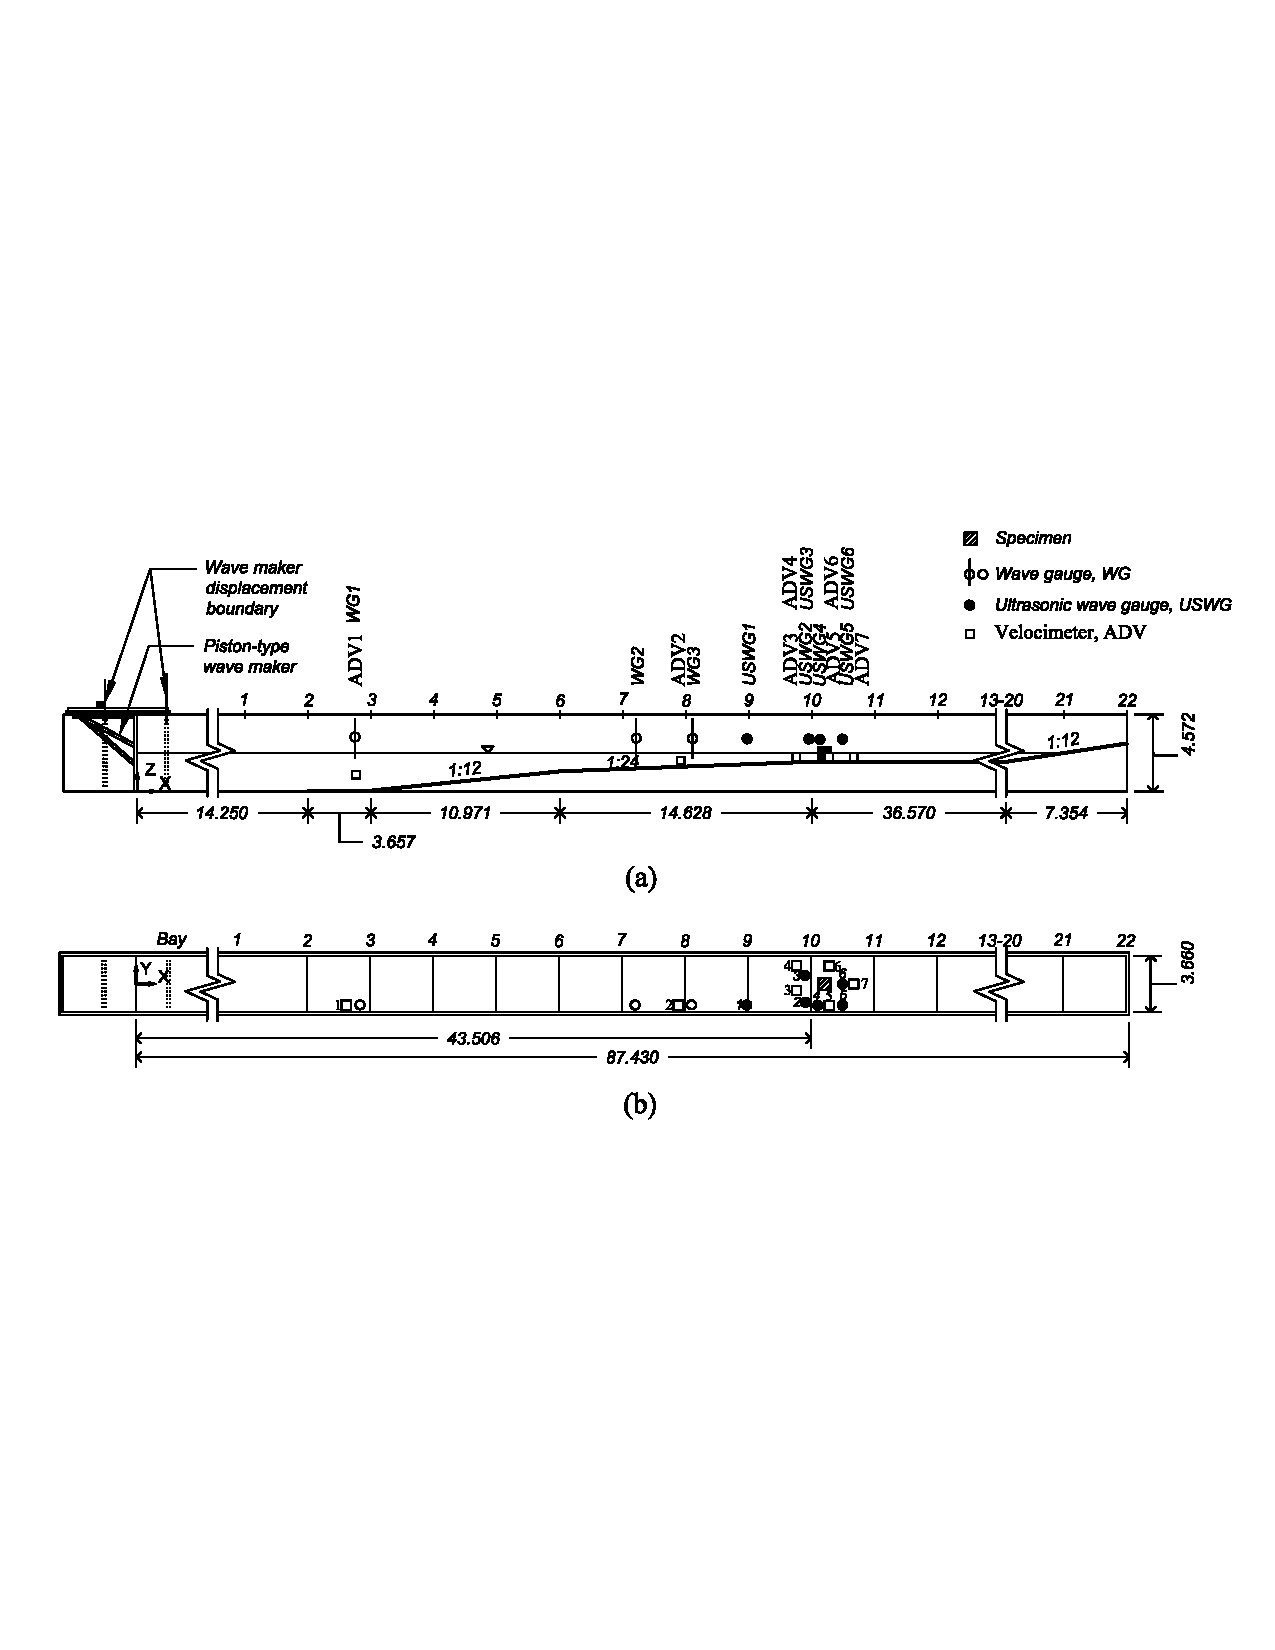
\includegraphics[width=1.2\textwidth]{WaveFlume.pdf}
  \caption{ Flume instrumentation adapted from \citep{winterTsunamiLikeWaveForces2020}.}
  \label{fig:waveflume}
\end{figure}

Wave paddle motions were prescribed using an error function displacement , which produces highly repeatable unbroken solitary waves. The wave velocity near the structure was measured using an Acoustic Doppler Velocimeter (ADV) and found to be approximately 1.3 m/s. Debris velocity, determined through video-based tracking, averaged around 0.8 m/s.
Repeatability was prioritized, as it ensured consistent wave conditions for comparing debris configurations. The still water level was set at 2.0 m, corresponding to a 0.25 m depth at the structure with no air gap beneath the base. The test structure was a 1.016 m square base × 0.615 m tall box constructed from sheet metal and steel framing (similar to \citep{winterTsunamiLikeWaveForces2020}), positioned 43.8 m from the wavemaker. It was mounted on low-friction bearings attached to a wall-mounted frame, allowing measurement of streamwise (x) and transverse (y) reactions.

The internal frame used hollow steel sections for stiffness, with additional aluminum-encased stiffeners to improve rotational resistance and load transfer. Eight load cells were installed: two streamwise, two transverse, and four vertical pancake cells, all sampled at 1200 Hz. Steel legs, 0.25 m in height, were placed below the structure but were not load bearing. Front and back view of the structure can be seen in Figure \ref{fig:teststructure_views}.

 \begin{figure}[htbp]
    \centering
    \begin{subfigure}[b]{0.48\textwidth}
        \centering
        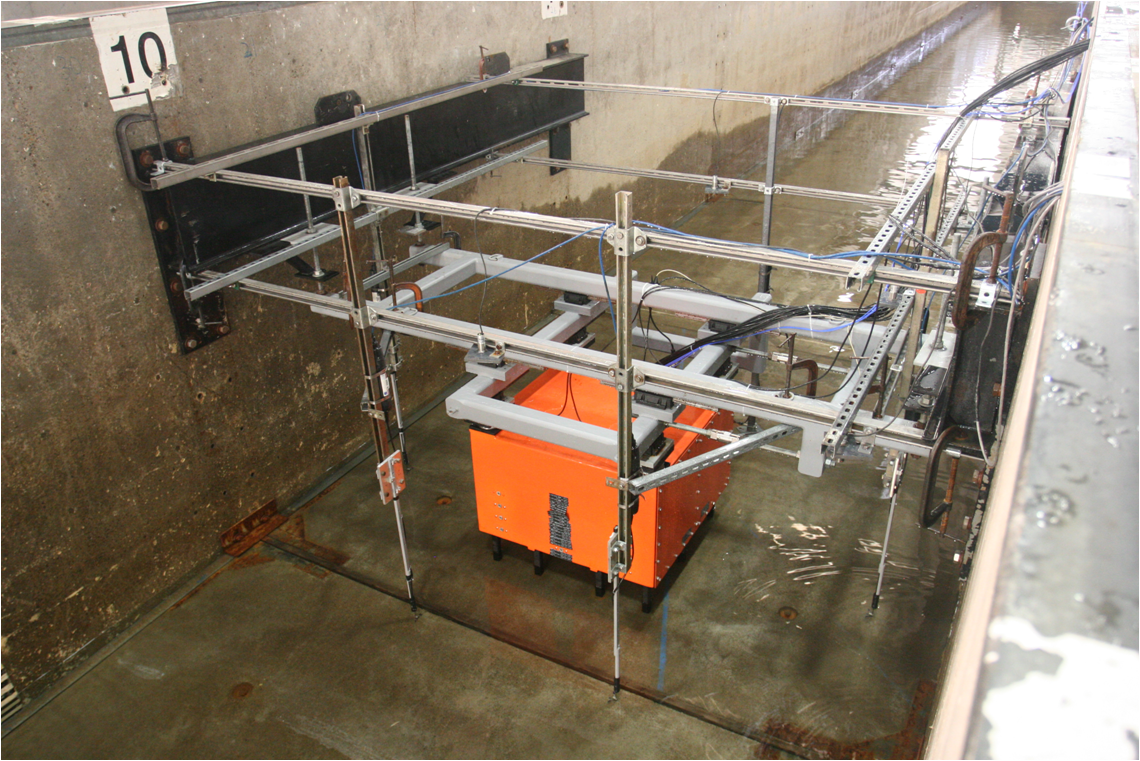
\includegraphics[width=\textwidth]{TestStructureFrontView.png}
        \caption{Front view of the test structure.}
        \label{fig:teststructure_front}
    \end{subfigure}
    \hfill
    \begin{subfigure}[b]{0.48\textwidth}
        \centering
        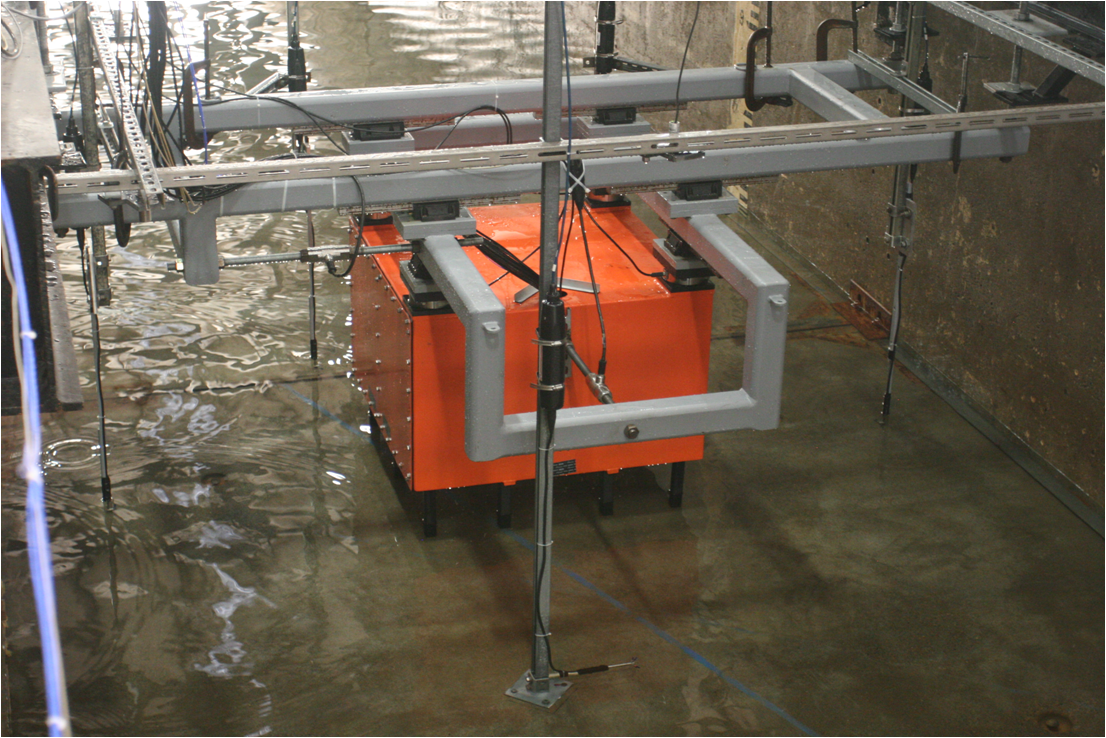
\includegraphics[width=\textwidth]{TestStructureBackView.png}
        \caption{Back view of the test structure.}
        \label{fig:teststructure_back}
    \end{subfigure}
    \caption{Front and back views of the test structure used in the debris impact experiments. 
    The front view shows the exposed face subjected to debris impact, while the back view highlights the instrumentation and load cell mounting.}
    \label{fig:teststructure_views}
\end{figure}

\begin{figure}[htbp]
    \centering
    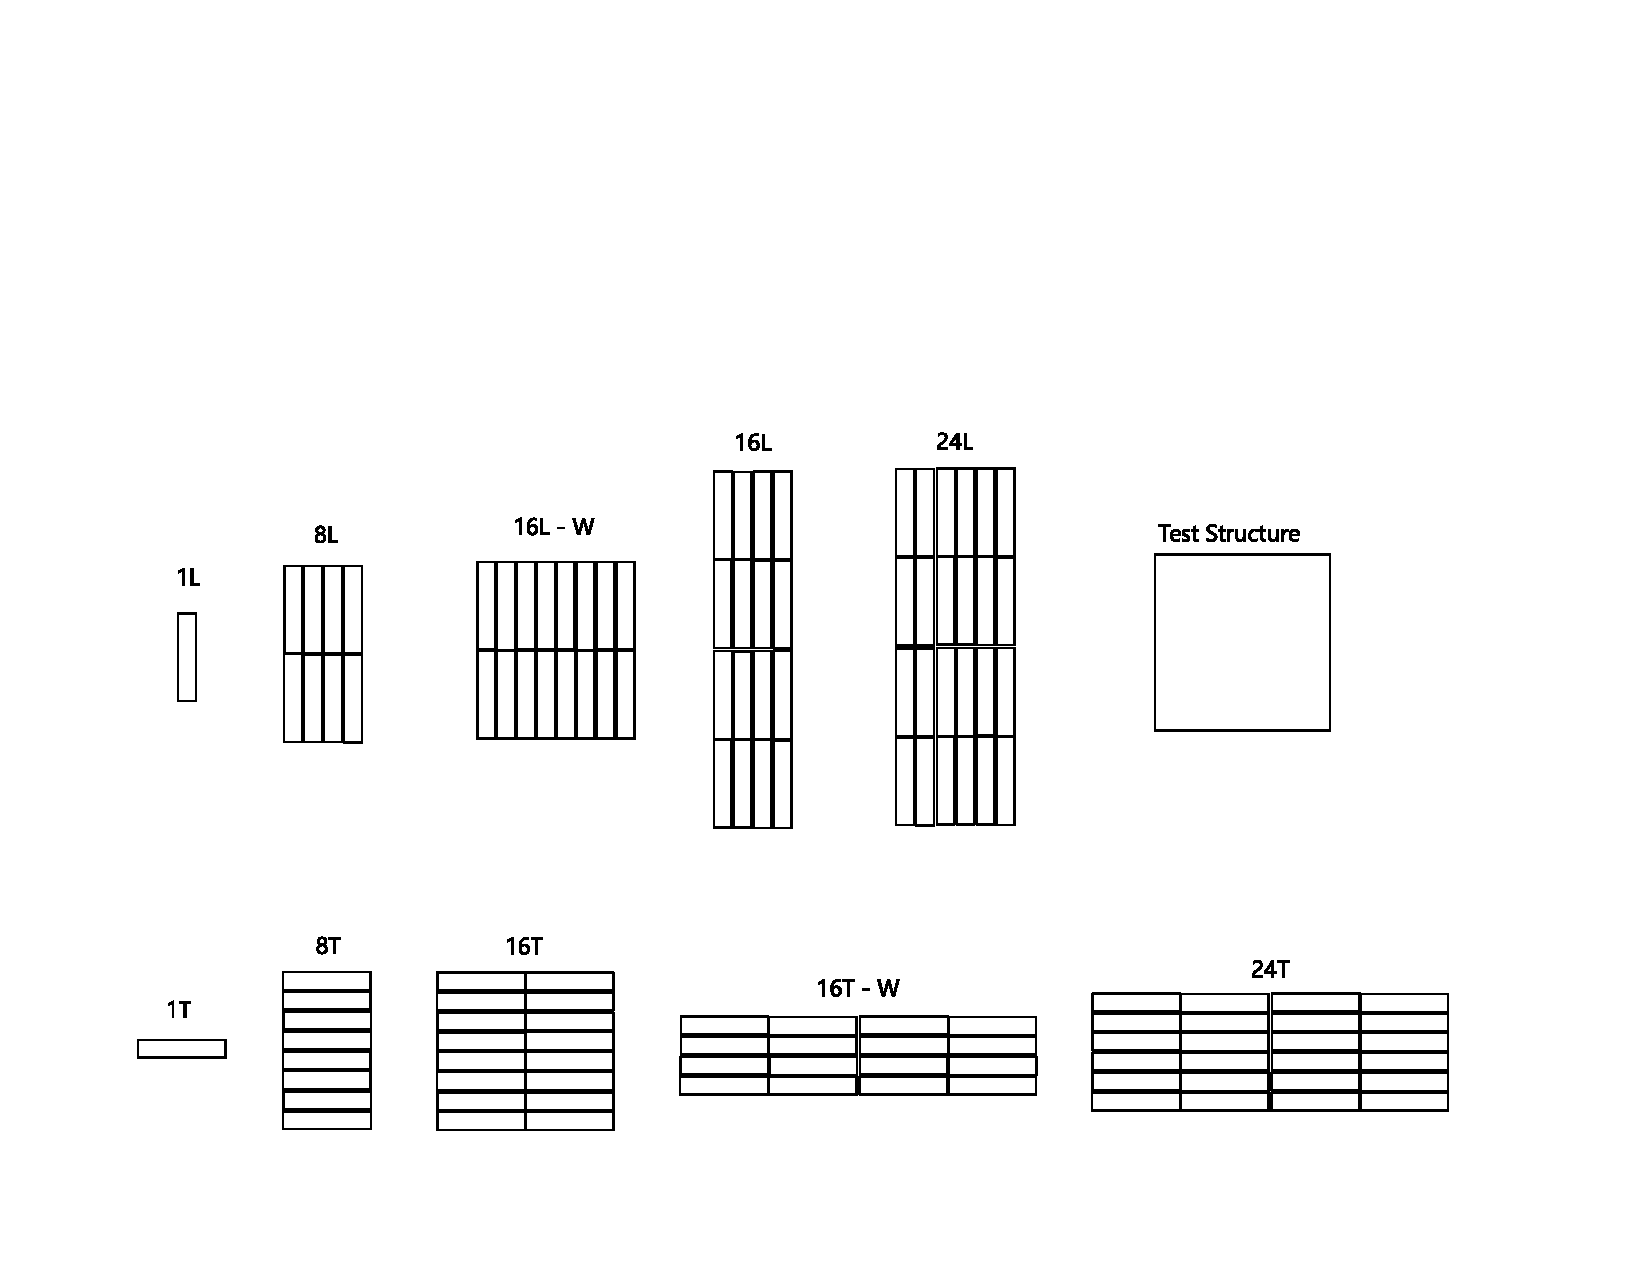
\includegraphics[width=1.4\textwidth]{Configurations.pdf}
    \caption{Regular configurations.}
    \label{fig:configurations}
\end{figure}


\begin{figure}[htbp]
    \centering
    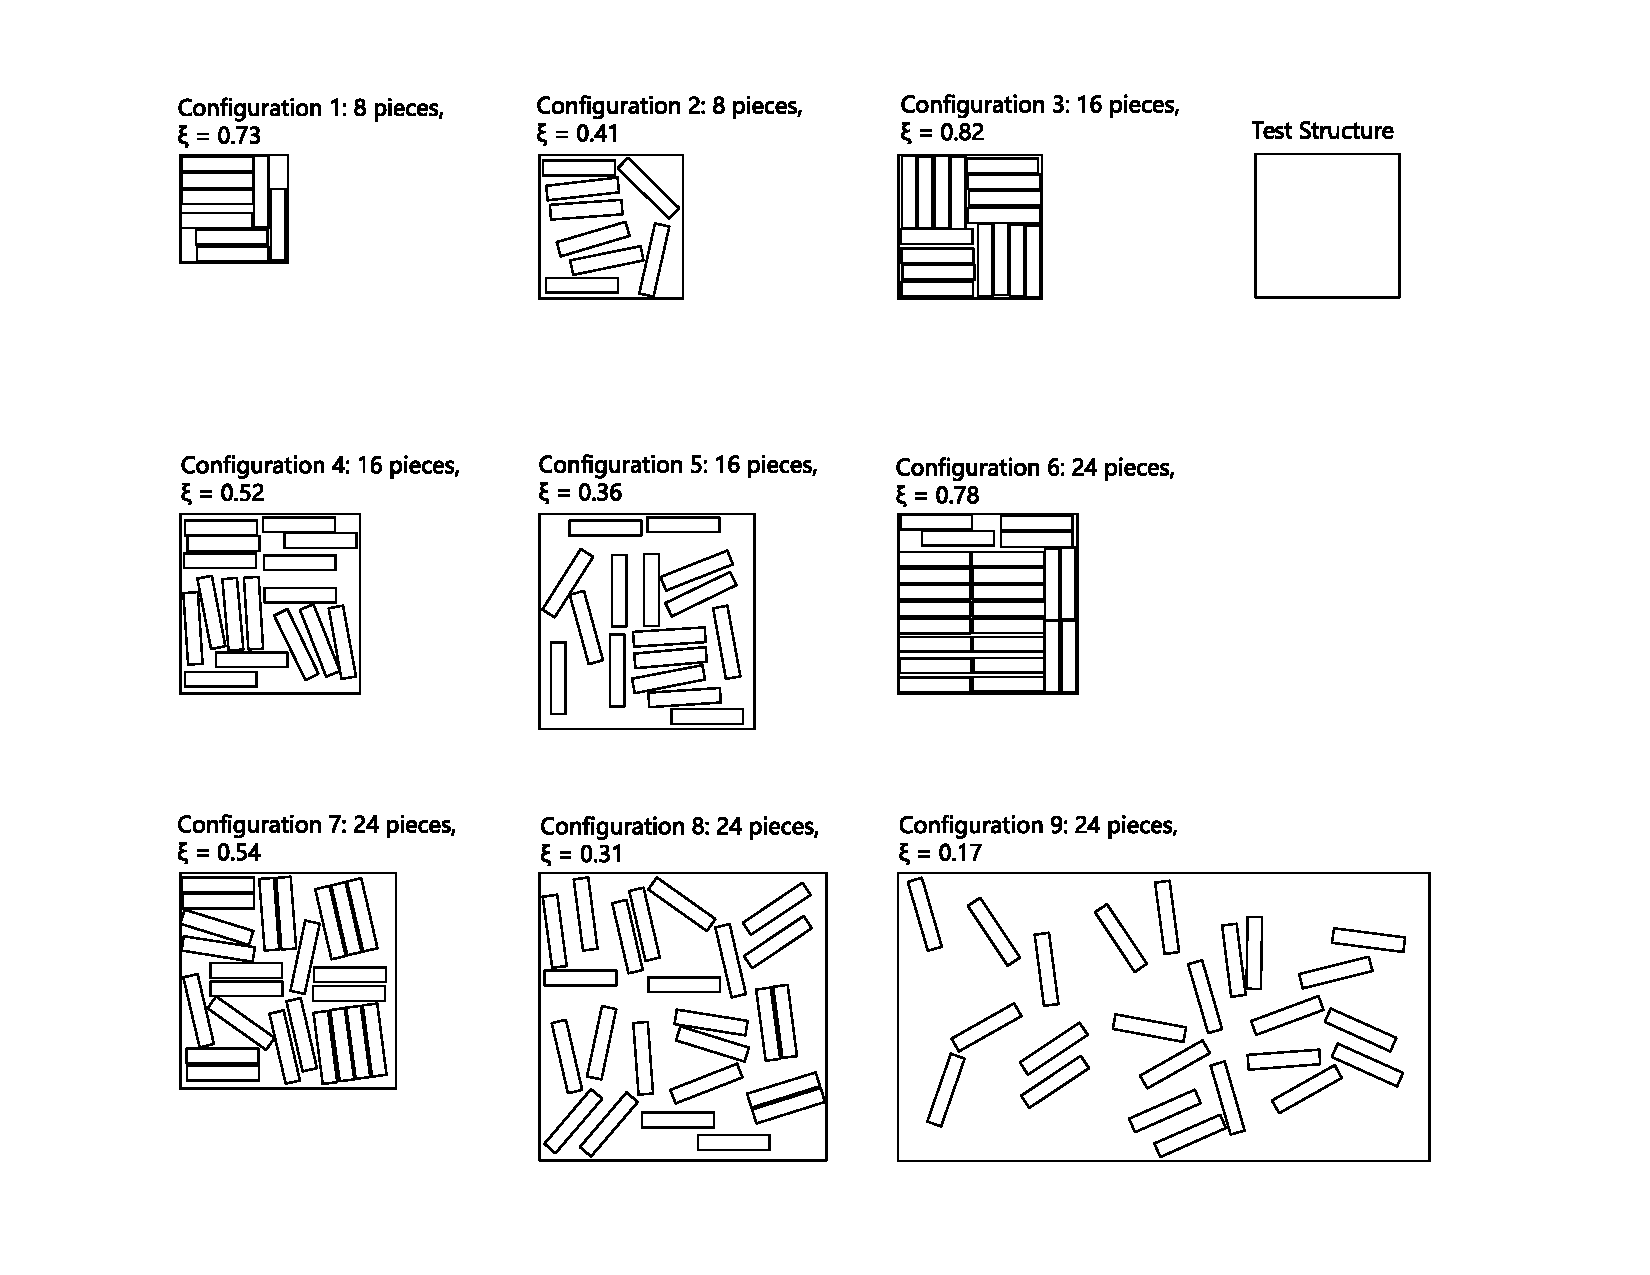
\includegraphics[width=1.5\textwidth]{configurations_rand.pdf}
    \caption{Random configurations.}
    \label{fig:configurations_random}
\end{figure}

The debris pieces were made of high-density polyethylene (HDPE), measuring 0.50 m × 0.051 m × 0.102 m and weighing approximately 2.52 kg. The submerged portion of each piece was 0.05 m, corresponding to its draft In-Water. Configurations included longitudinal, transverse, and random arrangements, with debris held 2 m upstream of the structure and released using lift frames modeled after \citet{Shekhar2020}. In addition to the single-size tests, multi-size configurations were also tested. These combined quarter-, half-, and full-sized debris pieces in varying proportions (see Table \ref{tab:multi_size_configs}) to examine the influence of packing ratio and size distribution on debris accumulation and loading behavior. 


\begin{table}[h!]
\centering
\caption{Regular debris configurations with longitudinal (L) and transverse (T) field widths. W denotes wide configurations.}
\small
\begin{tabular}{l r c r r}
\hline
\textbf{Config.} & \textbf{Count} & \textbf{Orient.} & \textbf{Length (m)} & \textbf{Width (m)} \\
\hline
0.25L & 0.25  & L & 0.125 & 0.102 \\
0.5L & 0.5  & L & 0.25 & 0.102 \\
0.5T & 0.5  & L &  0.102 & 0.25 \\
1L & 1  & L & 0.50 & 0.102 \\
1T & 1  & T & 0.102 & 0.50 \\
8L & 8  & L & 1.00 & 0.408 \\
8T & 8  & T & 0.816 & 0.50 \\
16T & 16 & T & 0.816 & 1.00 \\
16T-W & 16 & T & 0.408 & 2.00 \\
16L & 16 & L & 2.00 & 0.408 \\
16L-W & 16 & L & 1.00 & 0.816 \\
24L & 24 & L & 2.00 & 0.612 \\
24T-W & 24 & T & 0.612 & 2.00 \\
\hline
\end{tabular}
\label{tab:debris-configurations-compact}
\end{table}

\begin{table}[h!]
\centering
\caption{Random Debris Configurations and Longitudinal (L) and Transverse (T) field widths.}
\small
\begin{tabular}{l r c r r r}
\hline
\textbf{Config.} & \textbf{Count} & \textbf{Orient.} & \textbf{Length (m)} & \textbf{Width (m)} & \textbf{Packing ratio ($\xi$)} \\
\hline
8-0.73 & 8  & L & 0.75 & 0.75 & 0.73 \\
8-0.41 & 8  & L & 1.00 & 1.00 & 0.41 \\
16-0.82 & 16 & L & 1.00 & 1.00 & 0.82 \\
16-0.52 & 16 & L & 1.25 & 1.25 & 0.52 \\
16-0.36 & 16 & L & 1.50 & 1.50 & 0.36 \\
24-0.78 & 24 & L & 1.25 & 1.25 & 0.78 \\
24-0.54 & 24 & L & 1.50 & 1.50 & 0.54 \\
24-0.31 & 24 & L & 2.00 & 2.00 & 0.31 \\
24-0.17 & 24 & L & 3.70 & 2.00 & 0.17 \\
\hline
\end{tabular}
\label{tab:random-debris-compact}
\end{table}

\begin{table}[h!]
\centering
\caption{Summary of multi-size debris configurations. Multi-size debris tests combined quarter-, half- and full-sized pieces to study the effects of size distribution on debris accumulation and impact loading.}
{\small
\begin{tabular}{l r r r r r}
\hline
\textbf{Config.} & \textbf{Effective Debris Count}& \textbf{\# 0.25} & \textbf{\# 0.5 } & \textbf{\# 1} \\
\hline
8-0.73-M & 8   & 0  & 8  & 4 \\
8-0.41-M & 8  & 0  & 8  & 4 \\
16-0.82-M & 16 & 16 & 8  & 8 \\
16-0.52-M & 16  & 16 & 8  & 8 \\
16-0.36-M & 16  & 16 & 8  & 8 \\
24-0.78-M & 24  & 16 & 8  & 16 \\
24-0.54-M & 24  & 16 & 8  & 16 \\
\hline
\end{tabular}
}
\label{tab:multi_size_configs}
\end{table}



A total of 29 configurations were tested in the large wave flume. These included 10 regular configurations (5 transverse and 5 longitudinal) and 16 random configurations, of which 9 were single-sized and 7 were multi-sized. To assess the influence of debris size, additional tests were conducted using a single 0.25-size debris piece, as well as one transverse and one longitudinal configuration with 0.5-size debris. Each configuration was repeated for 10 independent trials. Furthermore, 32 In-Air swing tests were performed to characterize the structural response.

\section{Data Processing}

\begin{figure}[htbp] \centering 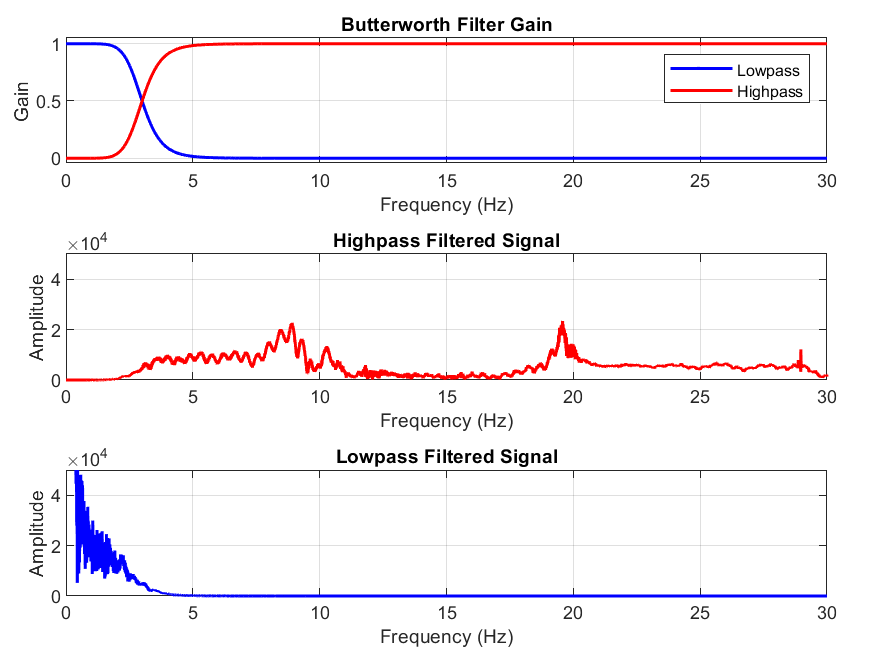
\includegraphics[width=0.9\textwidth]{high_low_pass.png} \caption{Force decomposition using Butterworth filters.} \label{fig:high_low_pass} \end{figure}

Force time histories were decomposed with Butterworth filters: high-pass filtering isolated short-duration impact peaks, while low-pass filtering captured sustained damming forces (Figure \ref{fig:high_low_pass}). A fourth-order Butterworth filter with a cutoff frequency of 2.5 Hz was applied. These parameters were selected based on preliminary analyses, which showed that this most effectively isolates the damming reaction forces. Examples (Figures \ref{fig:timehist_combined}–\ref{fig:timehist_damming_combined}) show the applied filter to the 1 L case and the 24 L case. 

\begin{figure}[h!]
    \centering
    \begin{subfigure}[b]{0.48\textwidth}
        \centering
        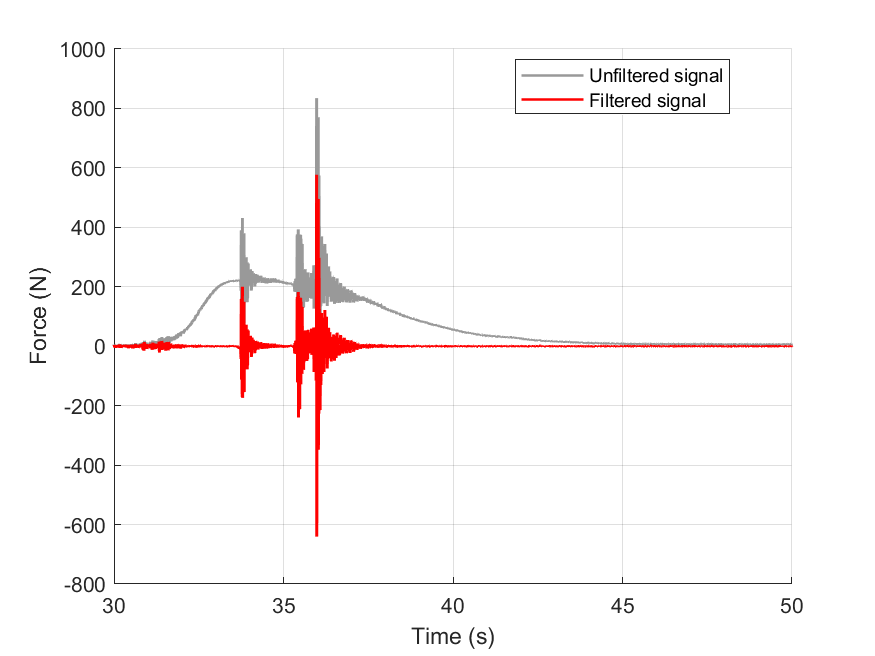
\includegraphics[width=\textwidth]{Reg_Lift_U_1_L_D__Masters_NHERIDeprisImpact2_goodtests_Reg_Lift_U_1_L_Trial04_Peak.png}
        \caption{1 L debris.}
        \label{fig:timehist_1L_peak}
    \end{subfigure}
    \hfill
    \begin{subfigure}[b]{0.48\textwidth}
        \centering
        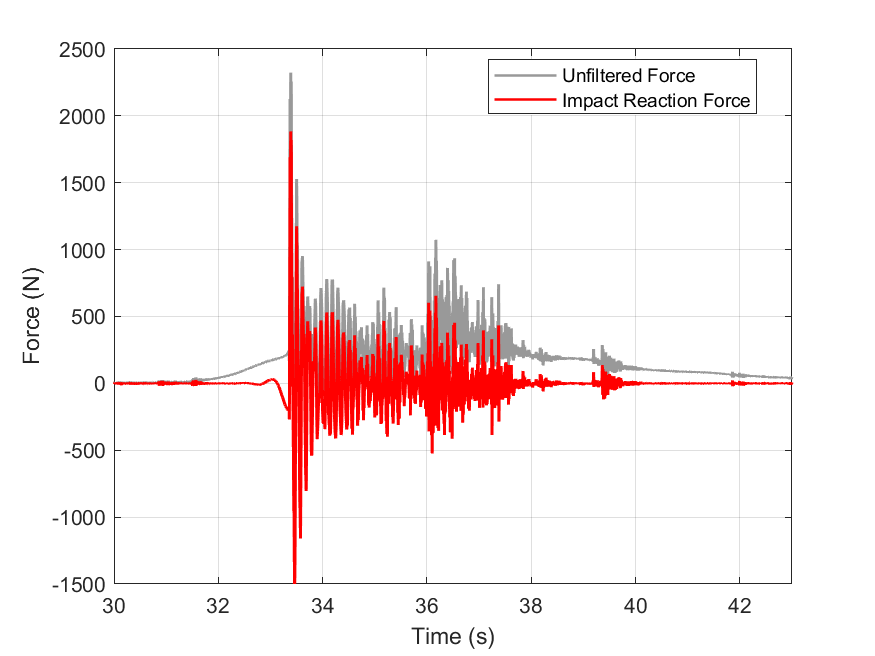
\includegraphics[width=\textwidth]{Reg_Lift_U_24_L_D__Masters_NHERIDeprisImpact2_goodtests_Reg_Lift_U_24_L_Trial04_Peak.png}
        \caption{24 L debris.}
        \label{fig:timehist_24L_peak}
    \end{subfigure}
    \caption{Reaction Force time histories filtered to isolate impact forces.}
    \label{fig:timehist_combined}
\end{figure}

\begin{figure}[h!]
    \centering
    \begin{subfigure}[b]{0.48\textwidth}
        \centering
        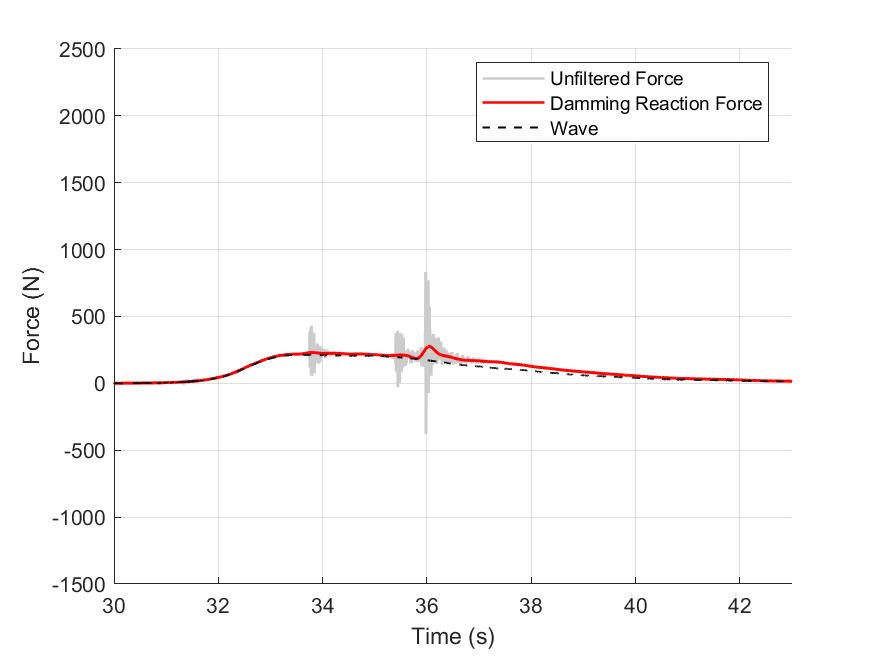
\includegraphics[width=\textwidth]{Reg_Lift_U_1_L_D__Masters_NHERIDeprisImpact2_goodtests_Reg_Lift_U_1_L_Trial04_Damming.png}
        \caption{1 L debris.}
        \label{fig:timehist_1L_damming}
    \end{subfigure}
    \hfill
    \begin{subfigure}[b]{0.48\textwidth}
        \centering
        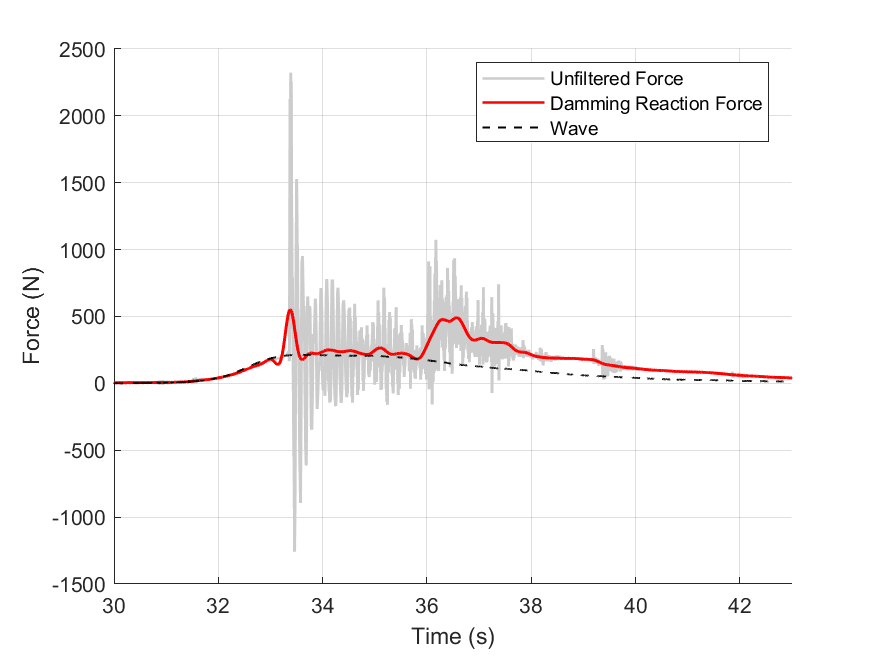
\includegraphics[width=\textwidth]{Reg_Lift_U_24_L_D__Masters_NHERIDeprisImpact2_goodtests_Reg_Lift_U_24_L_Trial04_Damming.png}
        \caption{24 L debris.}
        \label{fig:timehist_24L_damming}
    \end{subfigure}
    \caption{Reaction Force time histories filtered to isolate damming forces.}
    \label{fig:timehist_damming_combined}
\end{figure}


\subsection{Impact Identification}
Video evidence combined with filtered force records revealed that debris impacts occur in two distinct stages. The first stage is the initial unsubmerged impact, where debris pieces strike the structure immediately upon arrival (Figure~\ref{fig:first_impact}). These impacts are characterized by a sharp peak, particularly in longitudinal configurations. The debris pieces strike simultaneously and then scatter. The second stage consists of later submerged impacts, which arise when debris recirculates downstream and strikes the structure again under submerged conditions (Figure~\ref{fig:second_impact}). Unlike the first impact, these later impacts are more scattered, chaotic, and prolonged, especially in tests involving larger numbers of debris pieces. The distinction between first and later impacts proved consistent across all debris types and configurations, underscoring the need to treat these two stages as separate mechanisms in structural analysis.
Signal peaks were identified within predefined time intervals, determined from video observations of the debris motion. The first impact was detected within the initial time window, while subsequent impacts were identified by considering only times after the first impact and excluding the first peak impact. 

\subsection{Force Normalization}

Reaction forces were normalized using the following expressions:

\begin{equation}
    R_{\mathrm{impact,norm}} = 
    \frac{R_{\mathrm{impact}}}{R_{1L}}
    \label{eq:impact_norm}
\end{equation}

\begin{equation}
    R_{damming,\mathrm{norm}} = 
    \frac{R_{damming,\mathrm{max}} - R_{\mathrm{wave,max}}}
         {R_{\mathrm{wave,max}}}
    \label{eq:damming_norm}
\end{equation}

where \( R_{\mathrm{impact}} \) and \( R_{d,\mathrm{max}} \) are the measured impact and maximum damming forces, respectively, 
\( R_{1L} \) is the median impact force from the 1 L configuration, 
and \( R_{\mathrm{wave,max}} \) is the maximum reaction force from the unbroken wave-only reference case.


\begin{figure}[htbp]
    \centering
    \begin{subfigure}[b]{0.6\textwidth}
        \centering
        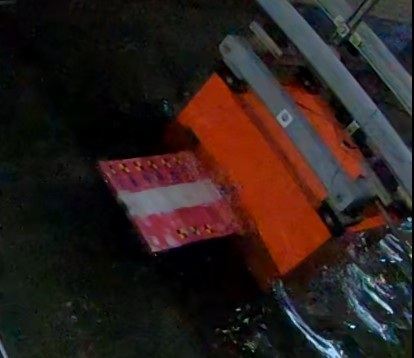
\includegraphics[width=\textwidth]{first_impact.jpg}
        \caption{First unsubmerged impact.}
        \label{fig:first_impact}
    \end{subfigure}
    \hfill
    
    \begin{subfigure}[b]{0.6\textwidth}
        \centering
        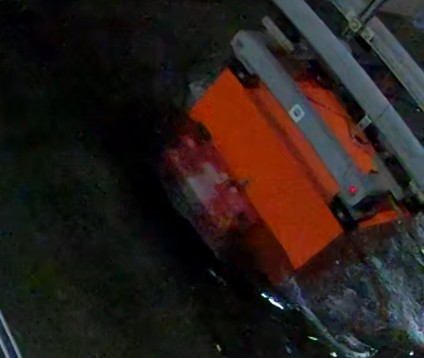
\includegraphics[width=\textwidth]{second_impact.jpg}
        \caption{Later submerged impact.}
        \label{fig:second_impact}
    \end{subfigure}
    \caption{Video capture of the 8 T impact event showing two distinct phases.}
    \label{fig:impact_combined}
    
\end{figure}

\section{Reaction Force Response to Single Debris Pieces} 
\subsection{Comparing In-Air to In-Water structural response} 
A total of 32 In-Air swing tests were carried out to characterize the dynamic behavior of the test structure. This behavior can be seen for both the In-Water and the In-Air tests in Figure \ref{fig:normalized_forces_structure}. Each test used a single debris piece of the same dimensions as the 1 L configurations, released from different drop-off heights. The reaction force signal recorded by the load cells at the back of the structure showed oscillatory behavior which corresponds to the dynamic response of several elements of the structure. Frequency spectra obtained through Fast Fourier Transform (FFT) analysis revealed three main amplification peaks, identified as the primary vibration modes of the structure, as summarized in Table \ref{tab:mode_summary}. After identifying the modes a bandwidth filter has been applied to the reaction force signal. After identifying the impacts a 0.5 seconds time window has been used to find the damping from the logarithmic decrement. These same modes were later confirmed for the 1 L configuration In-Water, where the natural frequencies decreased, which can be attributed to the added mass of water surrounding the structure. By isolating the modes in the reaction force signal, damping ratios were determined for each mode. The results showed an increase in damping when the structure was submerged, consistent with greater energy loss caused by fluid–structure interaction. The In-Air tests showed very low variability between trials in identifying the modes and damping ratios, while the in-water tests had higher standard deviations.


\begin{figure}[ht]
    \centering
    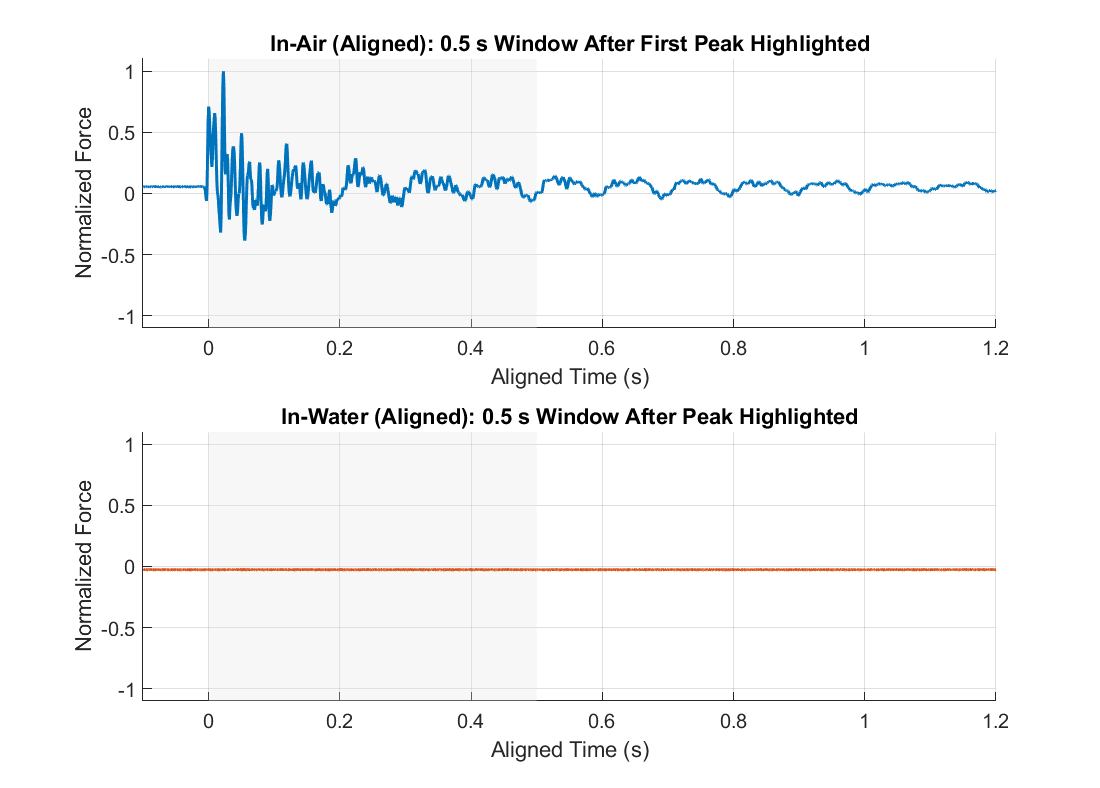
\includegraphics[width=\linewidth]{figures/plot_normalized_forces_in_air_vs_in_water_overlay.png}
    \caption{Normalized force responses for the In-Air test and 1 L configurations. Each subplot is normalized by its respective maximum force.}
    \label{fig:normalized_forces_structure}
\end{figure}


\begin{table}[ht]
\centering
\small
\begin{tabular}{c c c c c c c c c}
\hline
Mode & \multicolumn{4}{c}{In-Air (1L)} & \multicolumn{4}{c}{In-Water (1L)} \\
\cline{2-9}
 & $f$ [Hz] & Std $f$ [Hz] & $\zeta$ [\%] & Std $\zeta$ [\%] & $f$ [Hz] & Std $f$ [Hz] & $\zeta$ [\%] & Std $\zeta$ [\%] \\
\hline
Mode 1 & 9.830 & 0.045 & 2.08 & 0.37 & 9.266 & 0.136 & 5.38 & 1.73 \\
Mode 2 & 13.874 & 0.146 & 1.20 & 0.52 & 10.321 & 0.385 & 5.61 & 1.84 \\
Mode 3 & 19.940 & 0.084 & 0.91 & 0.20 & 19.582 & 0.160 & 1.66 & 0.23 \\
\hline
\end{tabular}

\caption{Median natural frequencies and damping ratios for In-Air (1L) and In-Water (1L) tests.}
\label{tab:mode_summary}
\end{table}


\subsection{In-Water - Single Debris Trials of Varying Size} 

All five single-piece configurations (10 trials each) were conducted to evaluate the effect of debris size on the reaction force. These tests aimed to characterize the behavior of individual debris pieces before examining group effects. Figure~\ref{fig:firstpeak_regular} shows the reaction force measured for single debris pieces with varying orientations. Higher variability is observed in the transverse orientation. 

\begin{figure}[htbp]
    \centering
    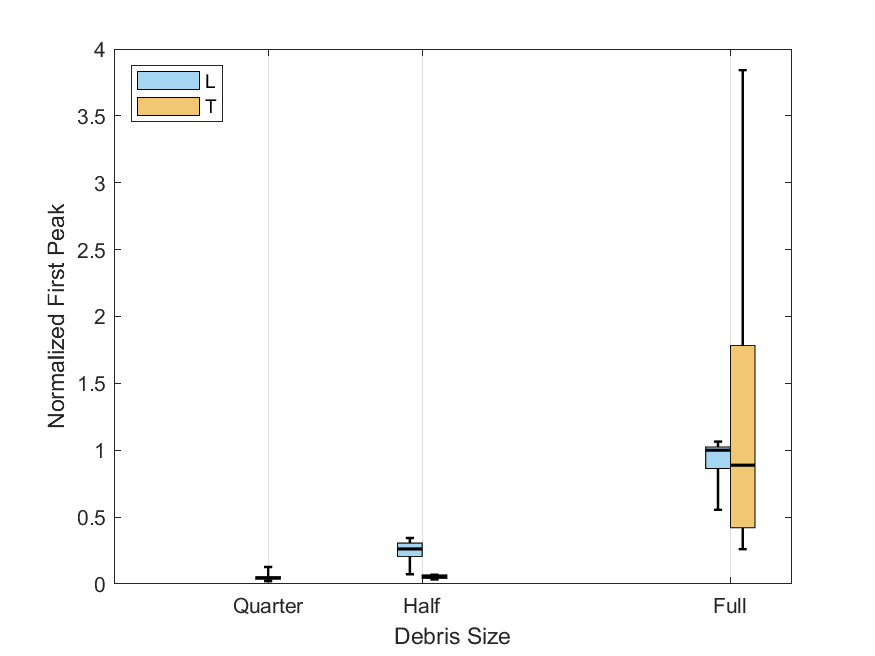
\includegraphics[width=\textwidth]{FirstPeak_Regular_SplitByTrial_single.png}
    \caption{Comparison of debris size at the first peak for regular configurations. The debris count in initial configurations is indicated within the boxplots.}
    \label{fig:firstpeak_regular}
\end{figure}


\subsection{Group effects}
\subsection{Regular Configurations}
\subsubsection{Impact Reaction Forces} 
Figure~\ref{fig:firstpeak_regular_split} and Figure~\ref{fig:laterpeak_regular_split} show the impact reaction forces from the first and second impacts. The boxplot whiskers represent the minimum and maximum values, the boxes indicate the interquartile range (IQR), and the solid line within each box marks the median value.
For specific cases such as the 24T-W and 16T-W tests, the width of the debris field exceeded the structure’s width. Consequently, not all debris pieces made contact with the structure. To address this limitation, the data was adjusted to reflect the amount of pieces impacting the structure.  Remapping makes the 24T-W case comparable to a 12T case, the total debris count still altered the flume hydrodynamics. This explains why the forces for the adjusted debris count appear lower than the corresponding smaller-group tests. 

In regular configurations, the first impact peaks scaled approximately linearly with the number of debris pieces (Figure~\ref{fig:firstpeak_regular_split}). This relationship was clear across both longitudinal and transverse configurations. Later impacts, by contrast, exhibited nonlinear behavior, showing growth that eventually saturated as debris counts increased (Figure~\ref{fig:laterpeak_regular_split}). This saturation suggests that once a certain number of pieces are present, additional debris no longer contributes significantly to impact loading because not all debris strike the structure simultaneously.

Longitudinal configurations consistently produced the highest impact forces, while transverse configurations yielded smaller peaks probably due to water cushioning.

\begin{figure}[htbp]
    \centering
    \begin{subfigure}[t]{0.9\textwidth}
        \centering
        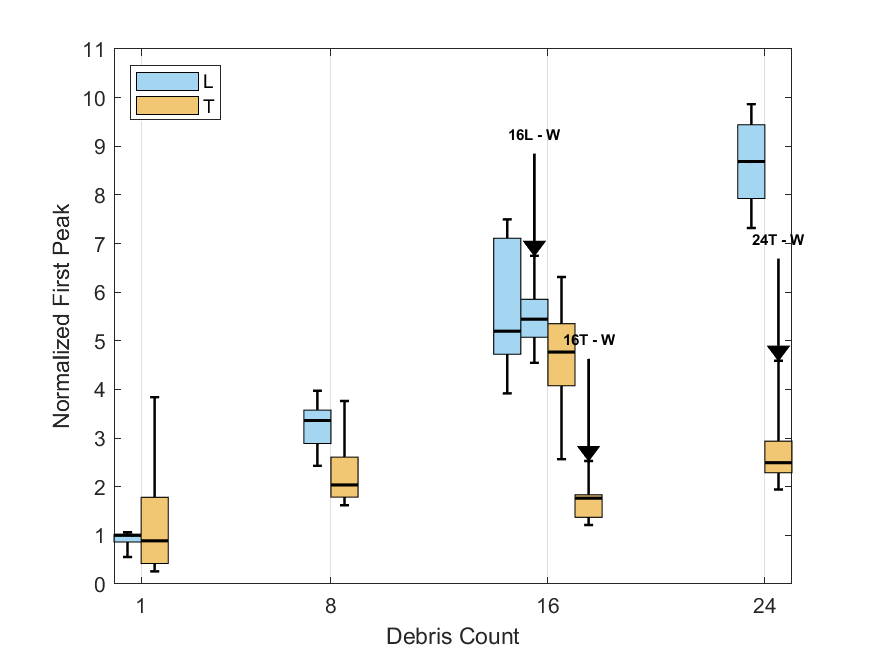
\includegraphics[width=\textwidth]{FirstPeak_Regular_SplitByTrial.png}
        \caption{Debris count in initial configurations as shown in Figure~\ref{fig:configurations}.}
        \label{fig:firstpeak_regular_original}
    \end{subfigure}
    \hfill
    \begin{subfigure}[t]{0.9\textwidth}
        \centering
        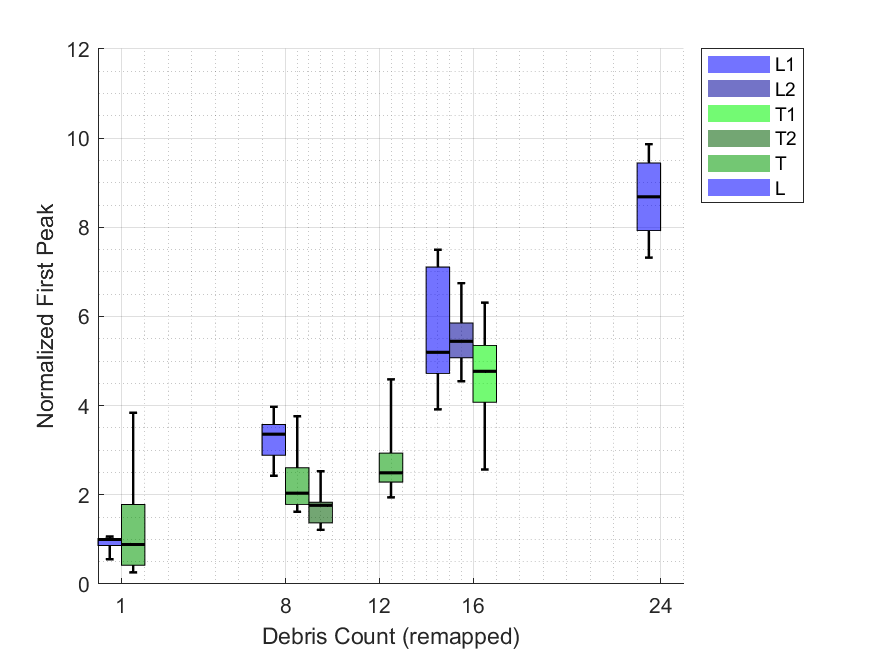
\includegraphics[width=\textwidth]{FirstPeak_Regular_RemappedT.png}
        \caption{Debris count adjusted using total of pieces impacting structure.}
        \label{fig:firstpeak_regular_remap}
    \end{subfigure}
    \caption{First peak forces in regular configurations for longitudinal and transverse orientations.}
    \label{fig:firstpeak_regular_split}
\end{figure}

\begin{figure}[htbp]
    \centering
    \begin{subfigure}[t]{0.9\textwidth}
        \centering
        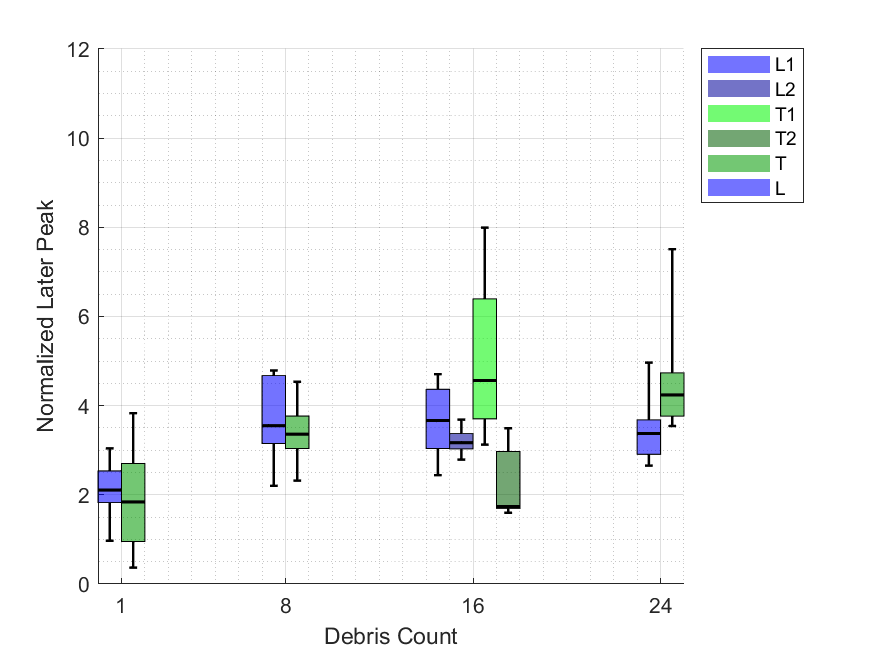
\includegraphics[width=\textwidth]{LaterPeak_Regular_SplitByTrial.png}
        \caption{Debris count in initial configurations as shown in Figure~\ref{fig:configurations}.}
        \label{fig:laterpeak_regular_original}
    \end{subfigure}
    \hfill
    \begin{subfigure}[t]{0.9\textwidth}
        \centering
        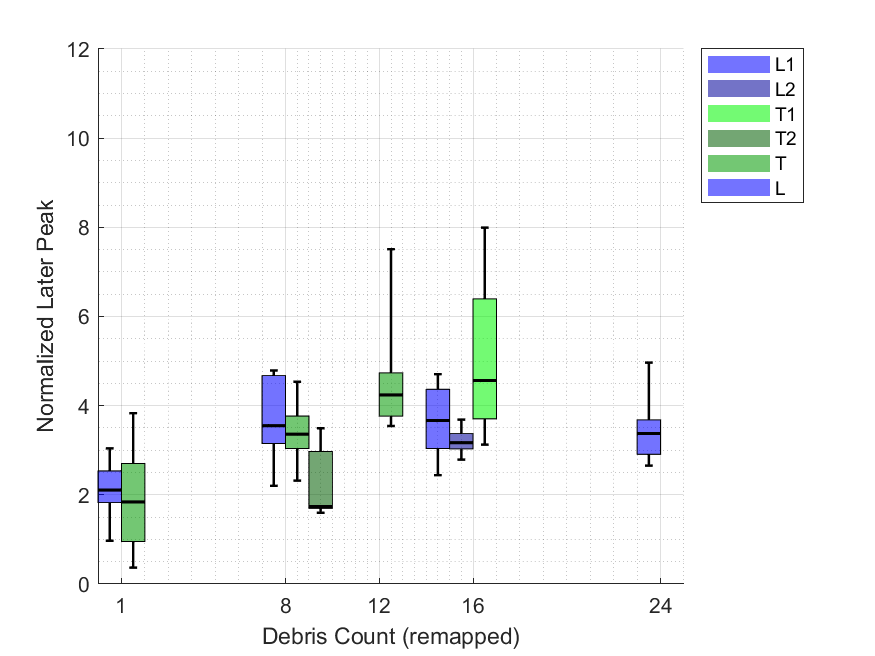
\includegraphics[width=\textwidth]{LaterPeak_Regular_RemappedT.png}
        \caption{Debris count adjusted using total of pieces impacting structure.}
        \label{fig:laterpeak_regular_remap}
    \end{subfigure}
    \caption{Later peak forces  in regular configurations for longitudinal and transverse orientations.}
    \label{fig:laterpeak_regular_split}
\end{figure}

\subsubsection{Damming Reaction Forces} 
Damming forces were extracted from low-pass filtered signals, capturing the sustained blockage loads. For regular debris configurations, transverse configurations produced higher damming forces than longitudinal configurations (Figure~\ref{fig:damming_regular_split}). This trend indicates that longitudinal configurations primarily influence impact peaks, whereas transverse configurations dominate sustained blockage forces. Nonlinear saturation was observed as debris counts increased: damming forces eventually plateaued, reflecting complete blockage conditions being achieved. 

\begin{figure}[htbp]
    \centering
    \begin{subfigure}[t]{0.9\textwidth}
        \centering
        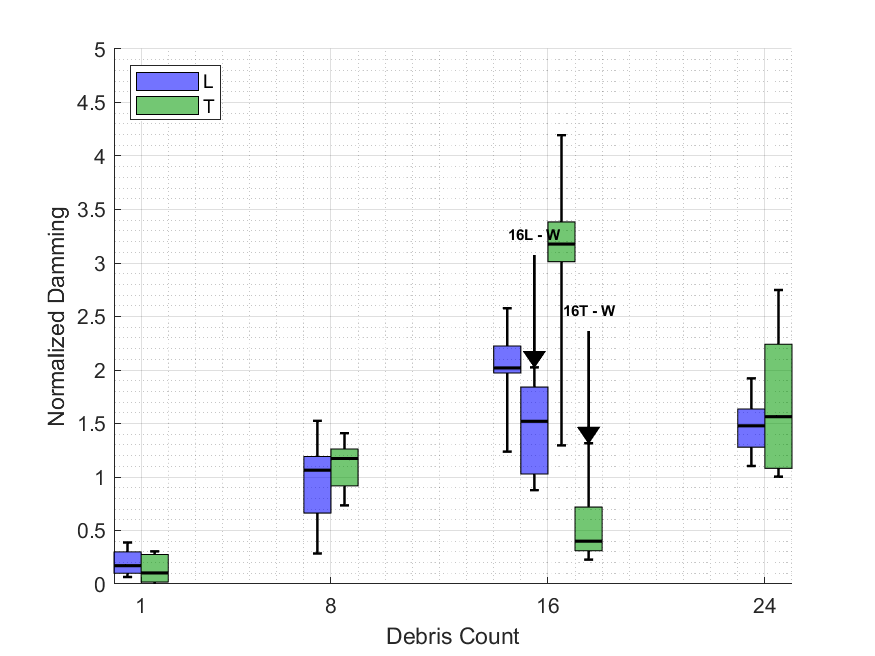
\includegraphics[width=\textwidth]{Damming_Regular_SplitByTrial.png}
        \caption{Debris count in initial configurations shown in Figure~\ref{fig:configurations}.}
        \label{fig:damming_regular_original}
    \end{subfigure}
    \hfill
    \begin{subfigure}[t]{0.9\textwidth}
        \centering
        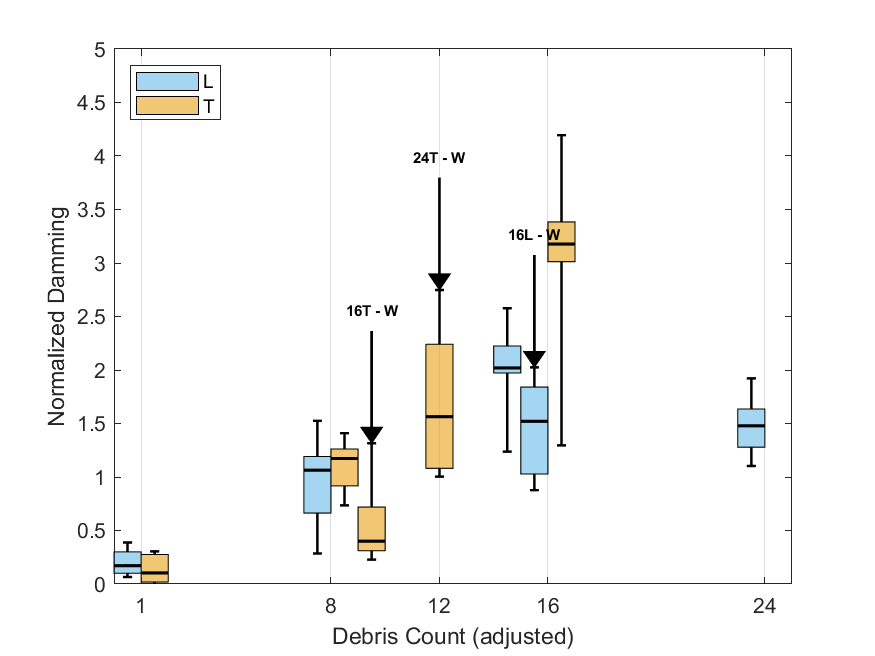
\includegraphics[width=\textwidth]{Damming_Regular_L_T_SplitByTrial_Remapped.png}
        \caption{Debris count adjusted using total of pieces impacting structure.}
        \label{fig:damming_regular_remap}
    \end{subfigure}
    \caption{Damming forces  in regular configurations for longitudinal and transverse orientations.}
    \label{fig:damming_regular_split}
\end{figure}

\subsection{Random Configurations}
Random debris fields with irregular orientations are analyzed by impact and damming forces as functions of debris count and packing ratio. Debris was initially arranged within a rectangular frame; at lower packing ratios, increasing the debris count caused the frame to extend beyond the structure’s width. Subsequent adjustments account for this using video-derived impact probabilities. The analysis includes corrected median values and a size-based assessment that isolates the contributions of the largest debris pieces in multi-size fields, revealing the limited influence of smaller pieces on structural loading.

\subsubsection{Impact Reaction Forces} 
Figure~\ref{fig:random_peaks_first} and Figure~\ref{fig:random_peaks_later} show the impact reaction forces from the first and later impacts, respectively, separated by packing ratio. The solid lines represent single-size debris configurations, while the dotted lines correspond to multi-size configurations. Boxplot whiskers indicate the minimum and maximum values, the boxes show the interquartile range (IQR), and the solid line within each box marks the median value.

Random debris configurations produced more scattered data compared to regular configurations. The peak magnitudes were generally smaller, but variability increased considerably. Multi-size fields consistently yielded lower impact magnitudes because smaller pieces contributed less momentum . Multi-sized vs. single-sized scenarios became more relevant with larger debris groups, as multiple debris pieces struck separately rather than together.

The unaltered gradient plots show these differences most clearly. In the first impact peaks, single-sized debris fields consistently yielded higher forces than multi-sized fields, and increasing packing ratio raised the magnitude of impact (Figure~\ref{fig:random_peaks_first}). Later impact peaks, occurring after initial contact and partial submergence, showed only a slight increase with debris count (Figure~\ref{fig:random_peaks_later}). In these later impacts, packing ratio effects were visible for single-sized debris fields but largely absent in multi-sized cases.

\begin{figure}[htbp]
    \centering
    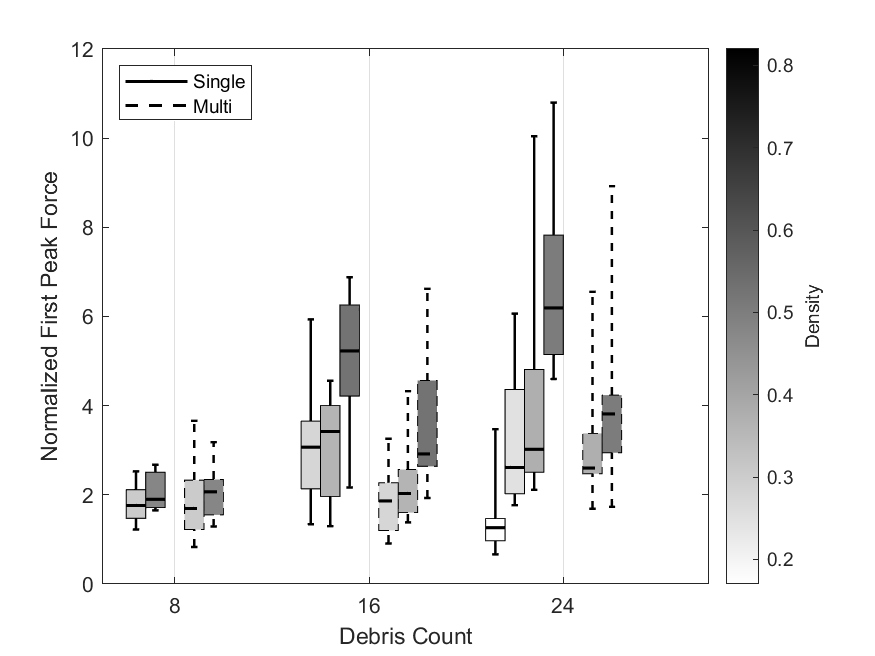
\includegraphics[width=0.9\textwidth]{First_Peak_Random_Single_vs_Multi_ByDensityGradient.png}
    \caption{First impact forces in random debris fields. Single-size debris yields higher peak forces than multi-size debris; lower packing ratio reduces peaks.}
    \label{fig:random_peaks_first}
\end{figure}

\begin{figure}[htbp]
    \centering
    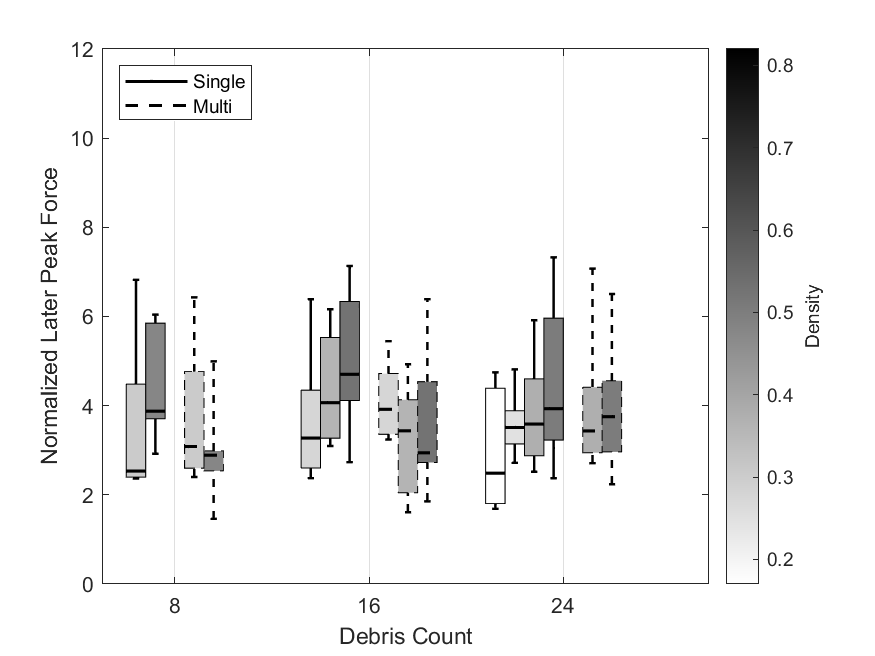
\includegraphics[width=0.9\textwidth]{Later_Peak_Random_Single_vs_Multi_ByDensityGradient.png}
    \caption{Later impact forces in random debris fields. Reaction forces increase slightly with debris count. packing ratio affects single-size debris fields but has negligible effect in multi-size fields.}
    \label{fig:random_peaks_later}
\end{figure}

An adjustment became necessary because debris frame exceeded the structure’s width when spanning higher densities for high debris counts. This geometry meant that not all pieces would impact the structure, and some pieces were effectively excluded from impact. Video analysis confirmed this by counting the number of debris pieces making contact with the structure. From these counts, an impact probability was derived, which decreased proportionally as the frame widened relative to the structure (Figure~\ref{fig:impact_probabilities}). To account for this effect, a linear correction was applied to all trials: the effective number of impacting pieces was defined as the nominal debris count multiplied by the ratio of structure width to Width of Debris Field. 

\begin{figure}[htbp]
    \centering
    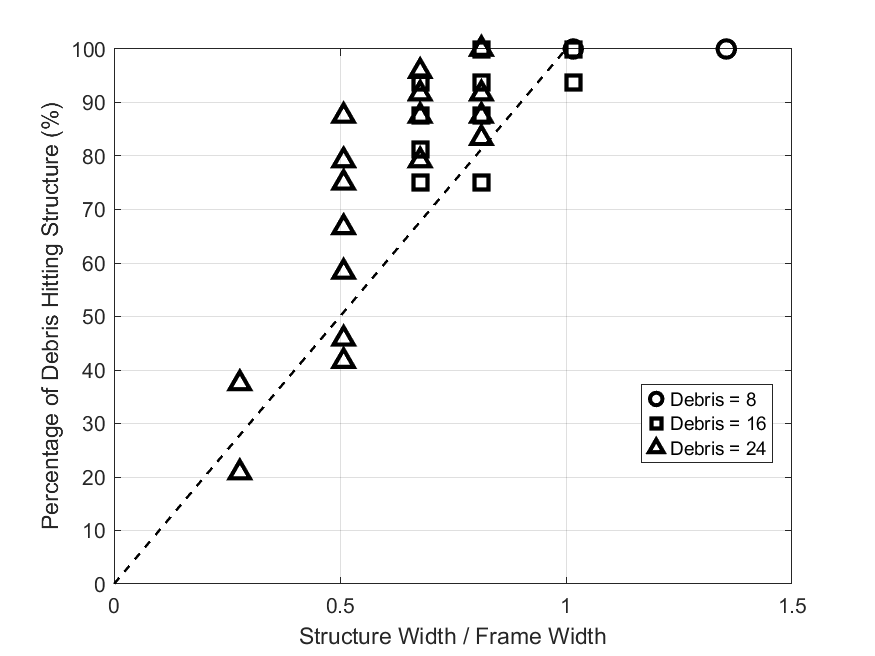
\includegraphics[width=0.9\textwidth]{Impact_probabilities.png}
    \caption{Impact probabilities across random trials. A larger frame-to-structure width ratio proportionally reduces the fraction of debris impacting the structure.}
    \label{fig:impact_probabilities}
\end{figure}

The corrected median plots reflect these adjustments. Figure~\ref{fig:random_first_median_adjusted} shows normalized first impact peaks after applying the width-based correction. Single-sized debris fields again produce higher forces than multi-sized fields, with forces rising until saturation as debris counts increase. In the analysis of multi-sized fields, an additional adjustment was performed to isolate the larger debris pieces equivalent to those in the single-sized configurations. The results indicate that these larger pieces generated only marginally higher impact peaks than the single-sized debris, whereas smaller pieces had a negligible effect. Thus, while smaller debris contributes to the loading response, peak forces are primarily governed by the larger pieces.

The same trends were observed in the later impact peaks (Figure~\ref{fig:random_later_median_adjusted}). Single-sized debris produced consistently stronger forces, while multi-sized debris showed weaker responses. Filtering for large pieces confirmed that smaller debris added only marginally to the total force.

\begin{figure}[htbp]
    \centering
    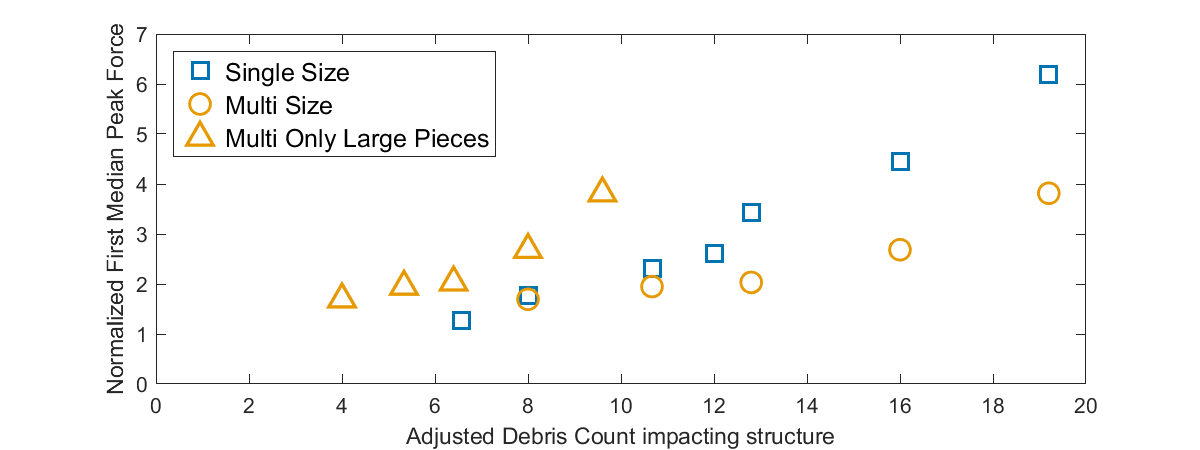
\includegraphics[width=0.75\textwidth]{First_Peak_Median_Single_vs_Multi_Adjusted.png}
    \caption{Median normalized first impact peaks in random fields, adjusted by structure width. Single-size debris fields produce higher peaks than multi-size fields. In multi-size fields, filtering out large pieces shows that smaller debris adds modest additional impact.}
    \label{fig:random_first_median_adjusted}
\end{figure}

\begin{figure}[htbp]
    \centering
    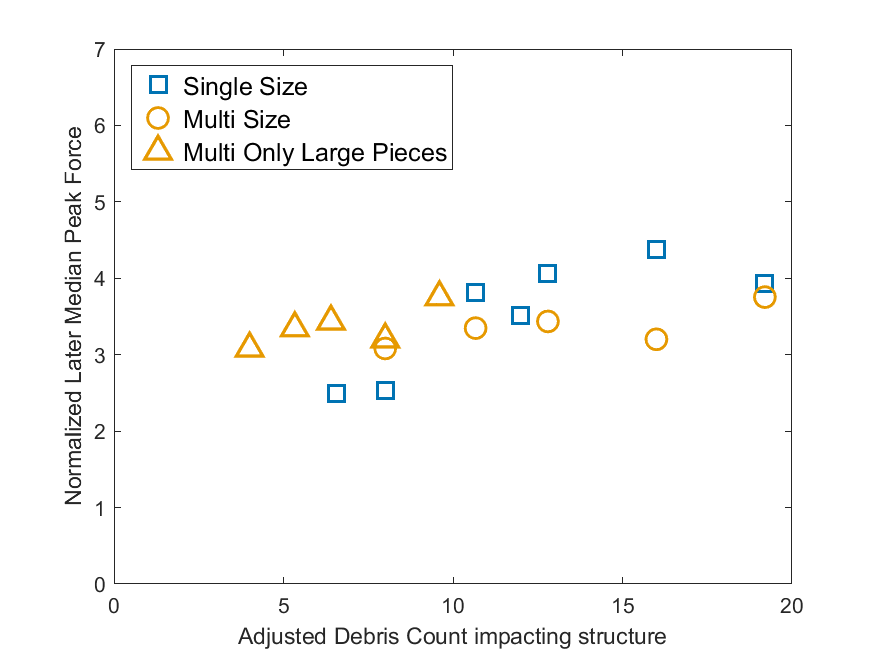
\includegraphics[width=0.75\textwidth]{Later_Peak_Median_Single_vs_Multi_Adjusted.png}
    \caption{Median normalized later impact peaks in random fields, adjusted by structure width. Single-size debris fields produce higher peaks than multi-size fields; in multi-size fields, smaller debris contributes only marginally when large pieces are filtered.}
    \label{fig:random_later_median_adjusted}
\end{figure}

\subsubsection{Damming Reaction Forces} 
In random configurations, damming forces followed a different pattern compared to regular configurations. The unaltered gradient plot (Figure~\ref{fig:random_damming_gradient}) shows that single-sized debris fields generated higher sustained loads than multi-sized fields, with packing ratio promoting stronger clustering. Multi-sized fields produced lower forces, probably because they allow more flow around obstacles and weaken packing ratio effects.

\begin{figure}[htbp]
    \centering
    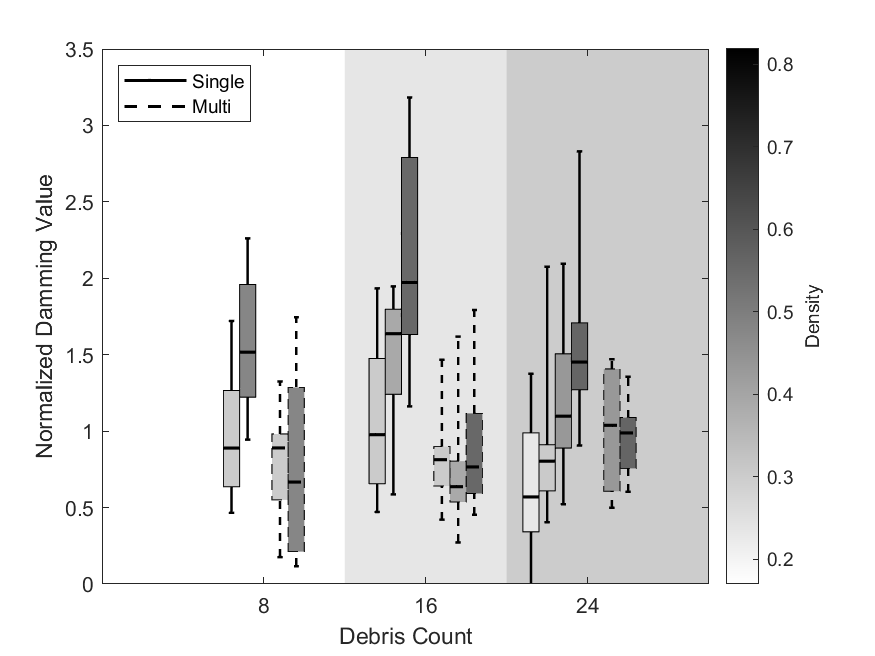
\includegraphics[width=0.9\textwidth]{Damming_Random_Single_vs_Multi_ByDensityGradient.png}
    \caption{Normalized damming forces in random debris fields. Single-size debris fields consistently produce higher forces than multi-size fields. packing ratio increases damming loads in single-size fields but has minimal effect in multi-size fields}
    \label{fig:random_damming_gradient}
\end{figure}

The corrected median values (Figure~\ref{fig:random_damming_median_adjusted}) show a noteworthy consistency: across all densities and debris counts, normalized damming forces remained close to a 100\% increase over baseline wave loading. This indicates that while packing ratio and debris size distribution influenced variability, the sustained force contribution of damming in random fields remained broadly similar across conditions. In other words, random configurations consistently doubled the baseline wave load, with single-size fields amplifying clustering effects and multi-size fields reducing them through blockage disruption.

\begin{figure}[htbp]
    \centering
    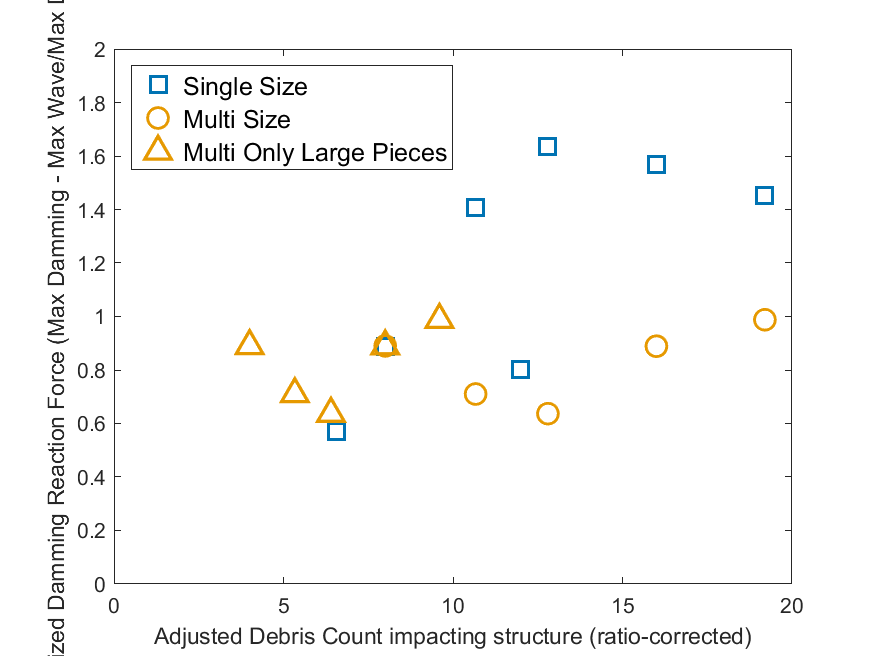
\includegraphics[width=0.75\textwidth]{Damming_Median_Single_vs_Multi_Adjusted.png}
    \caption{Median normalized damming forces in random fields, adjusted by structure width. Forces are roughly 100\% higher than wave-only loading, with packing ratio effects stronger in single-size fields and weaker in multi-size fields.}
    \label{fig:random_damming_median_adjusted}
\end{figure}


\section{Conclusions} The experiments demonstrate that debris orientation, size distribution, and packing ratio are all factors in determining the forces exerted on coastal structures. Longitudinal groups generated the largest impact peaks, while transverse groups dominated sustained damming forces. Random and multi-size fields generally produced smaller and more variable loads, highlighting their reduced capacity for synchronous impacts and stable blockages. 

\begin{itemize}
    \item \textbf{Debris orientation governs loading type:} Longitudinal configurationsconsistently produced the largest impact peaks due to synchronous debris strikes, while transverse configurations generated stronger sustained damming forces.
    
    \item \textbf{Debris size distribution influences variability:} Single-size debris fields produced higher and more consistent forces. Multi-size fields reduced both impact and damming magnitudes.
    
    \item \textbf{Random fields reduce predictability:} Random orientations yielded smaller average forces but introduced significantly greater variability. Larger pieces dominated responses in mixed fields, while smaller pieces contributed only marginally.
   
    \item \textbf{Synchrony of impacts:} Simultaneous contacts amplified impact forces, especially in longitudinal configurations where multiple debris pieces struck together. Random orientations reduced synchrony, leading to lower impact forces at higher debris counts.
    
    \item \textbf{Video-derived corrections refine debris momentum:} packing ratio did not account for the debris field width exceeding the structure. Video-based impact probabilities revealed a linear-proportional relationship between structure/Width of Debris Field and adjusted debris count. 


    \item \textbf{Two-stage impact behavior is consistent:} Initial unsubmerged impacts produced sharp, short-duration peaks, while later submerged impacts were more chaotic, prolonged, and nonlinear in their scaling with debris count.
\end{itemize}


\section{Limitations}
Several limitations of this study should be acknowledged. First, because of the high impact forces generated during the tests, it was not possible to directly record loads at the front of the structure. As a result, the measurements represent reaction forces transmitted through the structure, which inevitably include contributions from structural vibrations and cannot fully isolate the instantaneous impact loads. Second, the geometry of the flume influenced the flow conditions. In particular, confinement from the side walls amplified cushioning by the water, potentially altering the magnitude and duration of impacts compared to conditions in a coastal environment. Third, the relative widths of the debris fields and the test structure constrained the representativeness of certain configurations. When the debris field exceeded the structure width, only partial contact was achieved, requiring data adjustments to allow meaningful comparison across trials. Finally, the practical limits on the number of debris pieces that could be deployed restricted the parameter space explored in the experiments. While the tested cases captured a range of packing ratios, sizes, and orientations, the upper bound of debris group sizes was limited, leaving open the possibility that larger-scale accumulations could produce different scaling relationships. Addressing these constraints in future studies will be critical to improving the generalization of the results and to refining debris-impact models for coastal infrastructure design.

\bibliographystyle{plainnat}  
\bibliography{Thesis}
\section{Annex}
\begin{table}[h!]
\centering
\caption{Regular configurations: Impact Reaction Force (N)}
\begin{tabular}{lccccccc}
\toprule
\textbf{Debris Count} & \textbf{Orientation} & \textbf{Min} & \textbf{Q$_{25}$} & \textbf{Median} & \textbf{Q$_{75}$} & \textbf{Max} & \textbf{IQR} \\
\midrule
1 & L & 107.21 & 167.04 & 193.31 & 197.95 & 205.69 & 30.91 \\
1 & T & 50.38 & 81.25 & 171.64 & 344.53 & 742.75 & 263.29 \\
8 & L & 469.55 & 558.17 & 649.48 & 691.21 & 767.95 & 133.04 \\
8 & T & 313.19 & 345.13 & 393.83 & 504.21 & 727.34 & 159.08 \\
16 & L & 757.41 & 913.31 & 1004.70 & 1374.24 & 1449.02 & 460.93 \\
16 & L & 879.08 & 980.85 & 1052.44 & 1131.55 & 1304.36 & 150.70 \\
16 & T & 496.39 & 788.03 & 921.99 & 1034.63 & 1219.97 & 246.60 \\
16 & T & 234.63 & 265.07 & 340.92 & 354.42 & 489.07 & 89.34 \\
24 & L & 1414.91 & 1532.18 & 1678.85 & 1825.39 & 1907.21 & 293.21 \\
24 & T & 375.60 & 442.02 & 482.02 & 567.59 & 887.24 & 125.57 \\
\bottomrule
\end{tabular}
\end{table}

\begin{table}[h!]
\centering
\caption{Random Single-Sized debris configurations: Impact Reaction Force (N)}
\begin{tabular}{lccccccc}
\toprule
\textbf{Debris Count} & \textbf{Width (m)} & \textbf{Min} & \textbf{Q$_{25}$} & \textbf{Median} & \textbf{Q$_{75}$} & \textbf{Max} & \textbf{IQR} \\
\midrule
8 & 0.75 & 318.97 & 331.16 & 367.12 & 484.36 & 516.78 & 153.20 \\
8 & 1.00 & 236.24 & 284.84 & 340.64 & 408.94 & 488.05 & 124.10 \\
16 & 1.00 & 418.31 & 814.79 & 1010.74 & 1209.73 & 1330.04 & 394.94 \\
16 & 1.25 & 251.18 & 380.02 & 661.32 & 773.58 & 881.21 & 393.56 \\
16 & 1.50 & 258.88 & 412.69 & 593.04 & 706.10 & 1147.42 & 293.41 \\
24 & 1.25 & 888.86 & 994.75 & 1196.76 & 1512.85 & 2087.42 & 518.10 \\
24 & 1.50 & 408.07 & 484.46 & 584.12 & 930.06 & 1941.46 & 445.60 \\
24 & 2.00 & 341.88 & 391.34 & 505.48 & 843.64 & 1172.17 & 452.30 \\
24 & 3.65 & 128.40 & 187.59 & 244.38 & 283.56 & 671.54 & 95.97 \\
\bottomrule
\end{tabular}
\end{table}

\begin{table}[h!]
\centering
\caption{Random Multi-Sized debris configurations: Impact Reaction Force (N)}
\begin{tabular}{lccccccc}
\toprule
\textbf{Debris Count} & \textbf{Width (m)} & \textbf{Min} & \textbf{Q$_{25}$} & \textbf{Median} & \textbf{Q$_{75}$} & \textbf{Max} & \textbf{IQR} \\
\midrule
8 & 0.75 & 249.25 & 299.65 & 399.53 & 453.30 & 615.08 & 153.65 \\
8 & 1.00 & 160.32 & 235.97 & 327.54 & 450.15 & 707.13 & 214.18 \\
16 & 1.00 & 372.67 & 510.23 & 564.05 & 882.22 & 1279.70 & 371.99 \\
16 & 1.25 & 267.36 & 309.53 & 392.86 & 496.59 & 836.24 & 187.06 \\
16 & 1.50 & 175.67 & 231.79 & 359.92 & 438.89 & 630.04 & 207.10 \\
24 & 1.25 & 334.50 & 569.18 & 737.53 & 818.95 & 1725.19 & 249.77 \\
24 & 1.50 & 326.34 & 477.99 & 502.71 & 653.23 & 1266.47 & 175.24 \\
\bottomrule
\end{tabular}
\end{table}


\begin{table}[h!]
\centering
\caption{Regular configurations: Damming Reaction Force (N)}
\begin{tabular}{cccccccc}
\toprule
\textbf{Debris Count} & \textbf{Min} & \textbf{Q$_{25}$} & \textbf{Median} & \textbf{Q$_{75}$} & \textbf{Max} & \textbf{IQR} \\
\midrule
1 & 227.38 & 234.83 & 250.04 & 277.48 & 296.16 & 42.65 \\
1 & 213.19 & 217.32 & 235.43 & 272.40 & 278.61 & 55.08 \\
8 & 274.34 & 354.89 & 440.39 & 467.67 & 538.81 & 112.78 \\
8 & 370.29 & 409.17 & 463.73 & 482.75 & 514.36 & 73.58 \\
16 & 477.39 & 634.32 & 644.50 & 688.14 & 763.35 & 53.81 \\
16 & 400.58 & 432.87 & 537.93 & 606.28 & 645.49 & 173.41 \\
16 & 489.87 & 856.34 & 891.55 & 935.63 & 1108.87 & 79.28 \\
16 & 261.94 & 279.81 & 298.75 & 366.90 & 494.05 & 87.09 \\
24 & 448.78 & 486.28 & 529.06 & 562.54 & 623.60 & 76.26 \\
24 & 427.53 & 444.17 & 547.07 & 691.70 & 799.90 & 247.53 \\
\bottomrule
\end{tabular}
\end{table}

\begin{table}[h!]
\centering
\caption{Random Single-Sized debris configurations: Damming Reaction Force (N)}
\begin{tabular}{cccccccc}
\toprule
\textbf{Debris Count} & \textbf{Width (m)} & \textbf{Min} & \textbf{Q$_{25}$} & \textbf{Median} & \textbf{Q$_{75}$} & \textbf{Max} & \textbf{IQR} \\
\midrule
8 & 0.75 & 415.03 & 474.29 & 537.17 & 631.63 & 696.04 & 157.34 \\
8 & 1.00 & 312.70 & 349.20 & 403.20 & 483.63 & 580.62 & 134.43 \\
16 & 1.00 & 461.45 & 561.72 & 634.55 & 808.89 & 892.72 & 247.17 \\
16 & 1.25 & 338.60 & 478.26 & 562.87 & 597.09 & 628.93 & 118.83 \\
16 & 1.50 & 313.93 & 353.38 & 421.91 & 528.32 & 626.21 & 174.94 \\
24 & 1.25 & 406.77 & 484.70 & 523.35 & 578.01 & 817.46 & 93.31 \\
24 & 1.50 & 324.74 & 403.21 & 447.65 & 534.82 & 660.63 & 131.62 \\
24 & 2.00 & 299.56 & 343.45 & 384.97 & 407.82 & 656.45 & 64.37 \\
24 & 3.65 & 209.92 & 286.28 & 334.97 & 424.47 & 507.03 & 138.19 \\
\bottomrule
\end{tabular}
\end{table}

\begin{table}[h!]
\centering
\caption{Random Multi-Sized debris configurations: Damming Reaction Force (N)}
\begin{tabular}{cccccccc}
\toprule
\textbf{Debris Count} & \textbf{Width (m)} & \textbf{Min} & \textbf{Q$_{25}$} & \textbf{Median} & \textbf{Q$_{75}$} & \textbf{Max} & \textbf{IQR} \\
\midrule
8 & 0.75 & 238.19 & 258.69 & 355.83 & 488.00 & 585.86 & 229.32 \\
8 & 1.00 & 251.01 & 330.85 & 403.40 & 422.94 & 496.17 & 92.10 \\
16 & 1.00 & 310.06 & 339.79 & 376.89 & 451.63 & 595.93 & 111.83 \\
16 & 1.25 & 271.42 & 327.93 & 349.34 & 385.01 & 558.91 & 57.08 \\
16 & 1.50 & 303.26 & 350.25 & 387.00 & 405.22 & 526.45 & 54.97 \\
24 & 1.25 & 342.03 & 374.84 & 424.28 & 445.80 & 502.72 & 70.95 \\
24 & 1.50 & 319.81 & 342.89 & 435.02 & 513.73 & 527.27 & 170.85 \\
\bottomrule
\end{tabular}
\end{table}

\begin{table}[h!]
\centering
\caption{Regular configurations Single debris tests: Damming Reaction Force (N)}
\begin{tabular}{cccccccc}
\toprule
\textbf{Config.} & \textbf{Orient.} & \textbf{Min} & \textbf{Q$_{25}$} & \textbf{Median} & \textbf{Q$_{75}$} & \textbf{Max} & \textbf{IQR} \\
\midrule
0.25 &  & 4.21 & 6.93 & 8.46 & 10.64 & 24.63 & 3.71 \\
0.50 & L & 14.04 & 39.91 & 50.75 & 59.14 & 66.48 & 19.23 \\
0.50 & T & 6.71 & 8.07 & 10.78 & 13.11 & 13.38 & 5.04 \\
1.00 & L & 107.21 & 167.04 & 193.31 & 197.95 & 205.69 & 30.91 \\
1.00 & T & 50.38 & 81.25 & 171.64 & 344.53 & 742.75 & 263.29 \\
\bottomrule
\end{tabular}
\end{table}

\end{document}
